% ============================================================
%  INFORME FINAL — Programación Móvil
%  Gestión de Comandas
%  Universidad Mayor de San Simón
% ============================================================
\documentclass[12pt, a4paper]{report}

\usepackage[utf8]{inputenc}
\usepackage[T1]{fontenc}
\usepackage[spanish]{babel}

\usepackage[top=2.5cm, bottom=2.5cm, left=3cm, right=2.5cm]{geometry}

\usepackage{lmodern}
\usepackage{microtype}

\usepackage[dvipsnames,table]{xcolor}
\definecolor{umssblue}{RGB}{0, 51, 102}
\definecolor{umssred}{RGB}{180, 30, 30}
\definecolor{lightgray}{RGB}{245, 245, 245}
\definecolor{codegray}{RGB}{230, 230, 230}
\definecolor{huorange}{RGB}{210, 100, 20}

\usepackage{colortbl}


\usepackage{graphicx}
\usepackage{float}

\usepackage{booktabs}
\usepackage{tabularx}
\usepackage{longtable}
\usepackage{multirow}
\usepackage{array}
\usepackage{makecell}

\usepackage{enumitem}

\usepackage{listings}
\usepackage{lstautogobble}
\usepackage{amssymb}

\lstset{
  inputencoding=utf8,
  extendedchars=true,
  literate=
    {á}{{\'a}}1
    {é}{{\'e}}1
    {í}{{\'i}}1
    {ó}{{\'o}}1
    {ú}{{\'u}}1
    {Á}{{\'A}}1
    {É}{{\'E}}1
    {Í}{{\'I}}1
    {Ó}{{\'O}}1
    {Ú}{{\'U}}1
    {ñ}{{\~n}}1
    {Ñ}{{\~N}}1
    {ü}{{\"u}}1
    {Ü}{{\"U}}1
    {¿}{{?`}}1
    {¡}{{!`}}1
    {├}{{|}}1
    {└}{{\textbackslash}}1
    {│}{{|}}1
    {─}{{-}}1
}

\lstdefinestyle{sqlstyle}{
  language=SQL,
  backgroundcolor=\color{lightgray},
  basicstyle=\ttfamily\small,
  keywordstyle=\color{umssblue}\bfseries,
  stringstyle=\color{umssred},
  commentstyle=\color{gray}\itshape,
  numberstyle=\tiny\color{gray},
  numbers=left,
  stepnumber=1,
  frame=single,
  framesep=4pt,
  rulecolor=\color{gray!40},
  breaklines=true,
  autogobble=true,
  tabsize=2,
  showstringspaces=false,
}

\lstdefinestyle{tsstyle}{
  language=Java,
  backgroundcolor=\color{lightgray},
  basicstyle=\ttfamily\small,
  keywordstyle=\color{umssblue}\bfseries,
  stringstyle=\color{umssred},
  commentstyle=\color{gray}\itshape,
  numberstyle=\tiny\color{gray},
  numbers=left,
  stepnumber=1,
  frame=single,
  framesep=4pt,
  rulecolor=\color{gray!40},
  breaklines=true,
  autogobble=true,
  tabsize=2,
  showstringspaces=false,
  morekeywords={const,let,await,async,export,import,from,of,interface,type,uuid,text,boolean,decimal,integer,date,timestamptz,enum},
}

\lstdefinestyle{bashstyle}{
  backgroundcolor=\color{black!85},
  basicstyle=\ttfamily\small\color{white},
  frame=single,
  framesep=4pt,
  rulecolor=\color{black},
  breaklines=true,
  autogobble=true,
  tabsize=2,
}

\usepackage[hidelinks, colorlinks=false]{hyperref}
\usepackage{url}

\usepackage{fancyhdr}
\pagestyle{fancy}
\fancyhf{}
\fancyhead[L]{\small\textcolor{umssblue}{\textit{Facultad de Ciencias y Tecnologías}}}
\fancyhead[R]{\small\textcolor{umssblue}{\textit{Gestión de Comandas}}}
\fancyfoot[C]{\small\thepage}
\fancyfoot[R]{\small\textcolor{gray}{\textit{© 2026 UMSS. Cochabamba, Bolivia}}}
\renewcommand{\headrulewidth}{0.4pt}
\renewcommand{\footrulewidth}{0.4pt}

\usepackage{titlesec}
\titleformat{\chapter}[block]
  {\normalfont\Large\bfseries\color{umssblue}}
  {\thechapter.}{0.8em}{}
  [\vspace{0.2ex}\color{umssred}\titlerule]

\titleformat{\section}
  {\normalfont\large\bfseries\color{umssblue}}
  {\thesection}{0.8em}{}

\titleformat{\subsection}
  {\normalfont\normalsize\bfseries\color{umssblue!80}}
  {\thesubsection}{0.8em}{}

\titlespacing*{\chapter}{0pt}{-20pt}{20pt}
\titlespacing*{\section}{0pt}{10pt}{5pt}
\titlespacing*{\subsection}{0pt}{8pt}{4pt}

\setlength{\parindent}{0pt}
\setlength{\parskip}{6pt plus 2pt minus 1pt}

\usepackage{tcolorbox}
\tcbuselibrary{skins,breakable}
\newtcolorbox{notabox}{
  colback=umssblue!5,
  colframe=umssblue!50,
  fonttitle=\bfseries,
  title=Nota,
  breakable
}
\newtcolorbox{alertbox}{
  colback=umssred!5,
  colframe=umssred!60,
  fonttitle=\bfseries,
  title=Advertencia,
  breakable
}

\usepackage{verbatim}
\usepackage{fancyvrb}

\usepackage[labelfont=bf, textfont=it, labelsep=period]{caption}

\setcounter{tocdepth}{3}
\setcounter{secnumdepth}{3}

\usepackage{etoolbox}
\patchcmd{\chapter}{\thispagestyle{plain}}{\thispagestyle{fancy}}{}{}

\makeatletter
\renewcommand{\cleardoublepage}{\clearpage}
\makeatother

\raggedbottom
\begin{document}

\begin{titlepage}
  \thispagestyle{empty}
  \centering

  \begin{minipage}[c]{0.22\textwidth}
    \centering
    
\includegraphics[width=\textwidth]{img/logo_umss.png}
  \end{minipage}
  \hfill
  \begin{minipage}[c]{0.50\textwidth}
    \centering
    {\large\bfseries UNIVERSIDAD MAYOR DE SAN SIMÓN}\\[4pt]
    {\normalsize FACULTAD DE CIENCIAS Y TECNOLOGÍA}\\[4pt]
    {\normalsize CARRERA DE INFORMÁTICA}
  \end{minipage}
  \hfill
  \begin{minipage}[c]{0.22\textwidth}
    \centering
    
\includegraphics[width=\textwidth]{img/logo_fcyt.png}
  \end{minipage}

  \vspace{1cm}
  \textcolor{umssred}{\rule{\linewidth}{1.2pt}}
  \vspace{0.5cm}

  {\Huge\bfseries Ingeniería Informática}\\[12pt]
  {\LARGE\bfseries INFORME FINAL}\\[20pt]
  {\Large\bfseries\color{umssred} Gestión de Comandas}\\[6pt]
  {\normalsize Sistema móvil para la gestión de pedidos, ventas,\\
  gastos y reportes financieros en restaurantes}

  \vspace{0.5cm}
  \textcolor{umssred}{\rule{\linewidth}{0.8pt}}
  \vspace{0.5cm}

  \begin{tabular}{rl}
    \textbf{Materia:}  & Programación Móvil \\[4pt]
    \textbf{Docente:}  & Dr. Américo Fiorilo Lozada Ph.D. \\
  \end{tabular}

  \vspace{0.5cm}

  {\large\bfseries INTEGRANTES:}\\[8pt]
  \begin{tabular}{lll}
    \toprule
    \textbf{Nombre} & \textbf{Carrera} & \textbf{Rol} \\
    \midrule
    Acebey Zalazar Jimmy Randall    & Ing.\ Informática & Dev \\
    Cáceres Véliz Erick Alvaro      & Ing.\ Informática & Dev \\
    Revollo Bernal Amilcar Diego    & Ing.\ Informática & SM  \\
    Siles Espicho Adrian Eloy       & Ing.\ Informática & Dev \\
    Tinta Mamani Jairo Amado        & Ing.\ Informática & Dev \\
    \bottomrule
  \end{tabular}

  \vspace{1cm}

  \begin{tabular}{rl}
    \textbf{Carrera:} & Ing.\ Informática \\[4pt]
    \textbf{Fecha:}    & 10/04/2026 \\
  \end{tabular}

  \vfill

  {\large COCHABAMBA — BOLIVIA}
\end{titlepage}
\newpage

\tableofcontents
\newpage

\chapter{Resumen Ejecutivo}

El proyecto \textbf{Gestión de Comandas} consiste en el desarrollo de una aplicación
móvil integral diseñada para centralizar y gestionar operativamente los pedidos,
ventas, gastos y reportes financieros de restaurantes pequeños y medianos. La
plataforma aborda la problemática del registro manual en papel mediante una solución
tecnológica que permite a meseros y administradores operar en tiempo real desde
dispositivos Android, complementada con una carta digital pública y un sistema de
interacción directa del cliente desde su mesa.

\section{Problemática Resuelta}

La aplicación resuelve los principales desafíos identificados en la operación diaria
de restaurantes:

\begin{itemize}[leftmargin=1.5em]
  \item \textbf{Errores de cálculo} en el cierre diario de caja por registros manuales.
  \item \textbf{Dificultad de conciliación} entre ventas registradas e ingresos reales.
  \item \textbf{Ausencia de visibilidad financiera} en tiempo real para el administrador.
  \item \textbf{Procesos lentos} de verificación al final de cada turno.
  \item \textbf{Falta de trazabilidad} del estado de cada mesa durante el servicio.
  \item \textbf{Ausencia de un canal directo} entre cliente y mesero sin interrupciones físicas.
\end{itemize}

\section{Solución Implementada}

Se desarrolló una aplicación móvil nativa para Android con las siguientes
características principales:

\textbf{Arquitectura Técnica:}
\begin{itemize}[leftmargin=1.5em]
  \item \textit{Frontend móvil:} React Native con Expo SDK 52+
  \item \textit{Web (carta digital + sesión de cliente):} Expo Router (rutas públicas web)
  \item \textit{BaaS:} Supabase (PostgreSQL + Auth + Storage + Realtime)
  \item \textit{Lenguaje:} TypeScript
  \item \textit{Deploy:} Expo EAS Build + EAS Update (OTA)
\end{itemize}

\textbf{Funcionalidades Clave:}
\begin{itemize}[leftmargin=1.5em]
  \item Registro de pedidos con selección de platillos, mesa y método de pago.
  \item Vista en tiempo real del estado de mesas para el mesero.
  \item Notificaciones push cuando un pedido pasa a estado \textit{listo}.
  \item Carta digital pública accesible por QR sin necesidad de app ni registro.
  \item Sesión anónima del cliente por mesa: ver menú y llamar al mesero.
  \item Gestión completa del menú (CRUD + imágenes vía Supabase Storage).
  \item Registro de gastos operativos y generación de reportes financieros.
  \item Acceso diferenciado por rol: \texttt{waiter}, \texttt{admin}, \texttt{customer}.
\end{itemize}

\section{Metodología y Gestión}

El proyecto se desarrolló bajo la metodología ágil \textbf{Scrum}, organizado en
\textbf{3 sprints de 4 semanas} cada uno, con un equipo multidisciplinario de
5 integrantes que cumplieron roles específicos de desarrollo y gestión. Se utilizaron
herramientas modernas de colaboración como GitHub, Notion, Discord y Excalidraw
para garantizar una comunicación efectiva y un control de versiones robusto.
\chapter{Análisis del Proyecto}

\section{Objetivos}

\subsection{Objetivo General}

Desarrollar una aplicación móvil que permita registrar ventas, gestionar pagos,
controlar gastos, generar reportes financieros y visualizar el estado del servicio
en tiempo real en restaurantes pequeños y medianos.

\subsection{Objetivos Específicos}

\begin{enumerate}[leftmargin=1.8em]
  \item Permitir a los meseros registrar pedidos y pagos (efectivo o QR) desde
        dispositivos móviles.
  \item Implementar un sistema de gestión de menú con actualización de precios y
        disponibilidad en tiempo real.
  \item Registrar gastos operativos del restaurante (insumos, proveedores, etc.).
  \item Generar reportes automáticos de ingresos brutos, netos, egresos y ranking
        de platos más vendidos.
  \item Implementar acceso diferenciado por rol: \texttt{waiter}, \texttt{admin} y
        \texttt{customer}.
  \item Notificar a los meseros en tiempo real cuando un pedido está listo para
        ser entregado.
  \item Proveer al mesero una vista en tiempo real del estado de todas sus mesas.
  \item Exponer una carta digital pública accesible por QR para los clientes del
        restaurante.
  \item Permitir al cliente ver el menú completo con disponibilidad real y llamar
        al mesero desde su dispositivo, sin descargar ninguna app.
\end{enumerate}

\section{Problema o Necesidad Identificada}

Los restaurantes pequeños y medianos continúan registrando pedidos en papel, lo que
genera una serie de problemas operacionales recurrentes:

\begin{enumerate}[leftmargin=1.8em]
  \item \textbf{Errores de cálculo en caja:} El cierre diario depende de sumas
        manuales que son propensas a errores humanos.
  \item \textbf{Falta de conciliación:} Es difícil comparar ventas registradas con
        ingresos reales, especialmente cuando se mezclan pagos en efectivo y QR.
  \item \textbf{Sin visibilidad financiera en tiempo real:} El administrador no
        cuenta con datos inmediatos sobre el desempeño del día.
  \item \textbf{Procesos lentos de verificación:} Al final de cada turno, validar
        cada comanda consume tiempo significativo del personal.
  \item \textbf{Sin trazabilidad de mesas:} No existe un mecanismo para conocer
        el estado de cada mesa (libre, ocupada, con pedido listo) sin acercarse
        físicamente.
  \item \textbf{Sin canal cliente–mesero:} El cliente debe interrumpir al mesero
        para solicitar atención, lo que genera fricciones durante el servicio.
\end{enumerate}

\section{Contexto}

El sistema está diseñado para restaurantes de tamaño pequeño a mediano que buscan
modernizar su gestión operativa sin inversión en infraestructura de servidores
propios. El modelo BaaS (Backend as a Service) sobre Supabase permite desplegar
toda la solución sin administrar servidores, escalando automáticamente con la
demanda.

El público objetivo comprende:
\begin{itemize}[leftmargin=1.5em]
  \item \textbf{Meseros:} usuarios principales del día a día, con necesidad de
        interfaces rápidas e intuitivas.
  \item \textbf{Administradores:} responsables de la gestión del menú, gastos y
        reportes financieros.
  \item \textbf{Clientes en mesa:} usuarios ocasionales que interactúan mediante
        sesión anónima vía QR, sin necesidad de registro ni descarga de app.
\end{itemize}

\section{Requisitos Funcionales}

\begin{longtable}{>{\bfseries}p{1.5cm} p{11cm}}
  \toprule
  \textbf{ID} & \textbf{Requisito} \\
  \midrule
  \endhead
  RF-01 & Registro de pedidos con selección de platillos, mesa y método de pago. \\[3pt]
  RF-02 & Cálculo automático del total por venta. \\[3pt]
  RF-03 & Registro de gastos diarios por parte del administrador. \\[3pt]
  RF-04 & Actualización del menú (precios, disponibilidad, imágenes) en tiempo real. \\[3pt]
  RF-05 & Generación de reportes de ingresos brutos, netos y egresos (diario, semanal, mensual). \\[3pt]
  RF-06 & Reporte de platos más vendidos con ranking por período. \\[3pt]
  RF-07 & Acceso diferenciado: mesero solo accede a pedidos y mesas; admin accede a todo. \\[3pt]
  RF-08 & Notificaciones en tiempo real al mesero cuando el pedido pasa a estado \texttt{ready}. \\[3pt]
  RF-09 & Vista de estado de mesas para el mesero: pendiente, listo, entregado, libre. \\[3pt]
  RF-10 & Carta digital pública accesible mediante QR, sin necesidad de app ni registro. \\[3pt]
  RF-11 & El cliente puede escanear un QR por mesa para iniciar sesión anónima y ver el menú con disponibilidad real. \\[3pt]
  RF-12 & El cliente puede llamar al mesero desde su dispositivo, generando una notificación en tiempo real al mesero asignado. \\
  \bottomrule
  \caption{Requisitos Funcionales del Sistema}
\end{longtable}

\section{Requisitos No Funcionales}

\begin{longtable}{>{\bfseries}p{2cm} p{11cm}}
  \toprule
  \textbf{ID} & \textbf{Requisito} \\
  \midrule
  \endhead
  RNF-01 & Interfaz intuitiva con curva de aprendizaje mínima. \\[3pt]
  RNF-02 & Cifrado de datos sensibles (transacciones, sesiones). \\[3pt]
  RNF-03 & Escalable para múltiples sucursales. \\[3pt]
  RNF-04 & Disponibilidad alta con recuperación ante fallos. \\[3pt]
  RNF-05 & Compatible con Android. \\[3pt]
  RNF-06 & Procesamiento de pedidos sin latencia perceptible en horas pico. \\[3pt]
  RNF-07 & Actualizaciones sin interrupciones en el servicio (OTA vía Expo EAS Update). \\[3pt]
  RNF-08 & Carta digital accesible desde cualquier dispositivo con navegador web. \\[3pt]
  RNF-09 & La sesión del cliente en mesa no requiere registro ni descarga de aplicación. \\
  \bottomrule
  \caption{Requisitos No Funcionales del Sistema}
\end{longtable}

\subsection{Historias de Usuario}

Las historias de usuario representan los requerimientos funcionales del sistema
desde la perspectiva de los distintos actores involucrados, principalmente
administradores, meseros y clientes.

Cada historia describe una necesidad específica del usuario junto con el valor
que aporta al sistema, permitiendo organizar el desarrollo mediante iteraciones
incrementales.


\subsection{Setup e infraestructura}

% HU-01
\subsubsection*{HU-01 — Inicializar proyecto Expo con TypeScript y Expo Router}
\begin{table}[H]
\centering
\renewcommand{\arraystretch}{1.5}
\setlength{\arrayrulewidth}{0.8pt}
\arrayrulecolor{gray!60}
\begin{tabularx}{\textwidth}{|>{\bfseries}p{3.5cm}|X|>{\bfseries}p{3.5cm}|X|}
\hline
\rowcolor{huorange}
\multicolumn{1}{|l|}{\color{white}\bfseries HU-01} &
\multicolumn{3}{l|}{\color{white}\bfseries Inicializar proyecto Expo con TypeScript y Expo Router} \\
\hline
Estado & Sin empezar & Asignado & — \\
\hline
Esfuerzo & 2 puntos & Prioridad & Alta \\
\hline
Versión & 1.0 & Última edición & 2026-04-09 \\
\hline
\multicolumn{4}{|p{\dimexpr\textwidth-2\tabcolsep-2\arrayrulewidth}|}{%
  \cellcolor{lightgray!30}\textbf{Descripción} \par \vspace{4pt}
  Como desarrollador, quiero tener el proyecto base configurado con TypeScript y Expo Router para comenzar a construir sobre una estructura sólida y predecible desde el primer sprint.
} \\
\hline
\multicolumn{4}{|p{\dimexpr\textwidth-2\tabcolsep-2\arrayrulewidth}|}{%
  \textbf{Criterios de aceptación} \vspace{4pt}
  \begin{enumerate}[leftmargin=1.5em, itemsep=0pt, parsep=2pt, topsep=0pt]
    \item El proyecto compila y corre en Android sin errores ni advertencias críticas.
    \item Expo Router está configurado como sistema de navegación principal con soporte para grupos de rutas.
    \item \texttt{tsconfig.json} tiene el modo estricto activado (\texttt{"strict": true}).
    \item La estructura de carpetas sigue la convención \texttt{app/} con grupos \texttt{(auth)}, \texttt{(waiter)} y \texttt{(admin)}.
    \item Las variables de entorno están definidas en \texttt{.env} y excluidas del repositorio vía \texttt{.gitignore}.
    \item El proyecto tiene un \texttt{README.md} con instrucciones mínimas de instalación y ejecución local.
    \item El repositorio está inicializado en Git con una rama \texttt{main} protegida.
  \end{enumerate}
} \\
\hline
\end{tabularx}
\caption{HU-01: Configuración inicial del proyecto}
\end{table}

% HU-02
\subsubsection*{HU-02 — Configurar proyecto Supabase y variables de entorno}
\begin{table}[H]
\centering
\renewcommand{\arraystretch}{1.5}
\setlength{\arrayrulewidth}{0.8pt}
\arrayrulecolor{gray!60}
\begin{tabularx}{\textwidth}{|>{\bfseries}p{3.5cm}|X|>{\bfseries}p{3.5cm}|X|}
\hline
\rowcolor{huorange}
\multicolumn{1}{|l|}{\color{white}\bfseries HU-02} &
\multicolumn{3}{l|}{\color{white}\bfseries Configurar proyecto Supabase y variables de entorno} \\
\hline
Estado & Sin empezar & Asignado & — \\
\hline
Esfuerzo & 2 puntos & Prioridad & Alta \\
\hline
Versión & 1.0 & Última edición & 2026-04-09 \\
\hline
\multicolumn{4}{|p{\dimexpr\textwidth-2\tabcolsep-2\arrayrulewidth}|}{%
  \cellcolor{lightgray!30}\textbf{Descripción} \par \vspace{4pt}
  Como desarrollador, quiero tener el cliente Supabase conectado al proyecto para poder consumir todos sus servicios desde la aplicación móvil.
} \\
\hline
\multicolumn{4}{|p{\dimexpr\textwidth-2\tabcolsep-2\arrayrulewidth}|}{%
  \textbf{Criterios de aceptación} \vspace{4pt}
  \begin{enumerate}[leftmargin=1.5em, itemsep=0pt, parsep=2pt, topsep=0pt]
    \item \texttt{supabase-js} v2 está instalado como dependencia del proyecto.
    \item \texttt{lib/supabase.ts} expone el cliente autenticado con la \texttt{SUPABASE\_URL} y \texttt{SUPABASE\_ANON\_KEY}.
    \item \texttt{lib/supabase-public.ts} expone un cliente separado para uso anónimo en carta digital y sesión de cliente.
    \item El archivo \texttt{.env} está incluido en \texttt{.gitignore} y se provee un \texttt{.env.example} con las claves vacías.
  \end{enumerate}
} \\
\hline
\end{tabularx}
\caption{HU-02: Configuración del cliente Supabase}
\end{table}

% HU-03
\subsubsection*{HU-03 — Crear migración de esquema inicial de la base de datos}
\begin{table}[H]
\centering
\renewcommand{\arraystretch}{1.5}
\setlength{\arrayrulewidth}{0.8pt}
\arrayrulecolor{gray!60}
\begin{tabularx}{\textwidth}{|>{\bfseries}p{3.5cm}|X|>{\bfseries}p{3.5cm}|X|}
\hline
\rowcolor{huorange}
\multicolumn{1}{|l|}{\color{white}\bfseries HU-03} &
\multicolumn{3}{l|}{\color{white}\bfseries Crear migración de esquema inicial de la base de datos} \\
\hline
Estado & Sin empezar & Asignado & — \\
\hline
Esfuerzo & 3 puntos & Prioridad & Alta \\
\hline
Versión & 1.0 & Última edición & 2026-04-09 \\
\hline
\multicolumn{4}{|p{\dimexpr\textwidth-2\tabcolsep-2\arrayrulewidth}|}{%
  \cellcolor{lightgray!30}\textbf{Descripción} \par \vspace{4pt}
  Como desarrollador, quiero tener todas las tablas del sistema creadas mediante migraciones versionadas para mantener el historial del esquema y poder replicar el entorno en cualquier momento.
} \\
\hline
\multicolumn{4}{|p{\dimexpr\textwidth-2\tabcolsep-2\arrayrulewidth}|}{%
  \textbf{Criterios de aceptación} \vspace{4pt}
  \begin{enumerate}[leftmargin=1.5em, itemsep=0pt, parsep=2pt, topsep=0pt]
    \item La migración \texttt{001\_schema.sql} crea las tablas: \texttt{restaurants}, \texttt{tables}, \texttt{users}, \texttt{menu\_items}, \texttt{orders}, \texttt{order\_items}, \texttt{payments}, \texttt{expenses} y \texttt{table\_calls}.
    \item Todos los enums del sistema están definidos: \texttt{order\_status}, \texttt{payment\_method}, \texttt{payment\_status} y \texttt{user\_role}.
    \item La migración se ejecuta sin errores en un proyecto Supabase limpio.
    \item El tipo de dato \texttt{decimal(10,2)} se usa para todos los campos monetarios.
  \end{enumerate}
} \\
\hline
\end{tabularx}
\caption{HU-03: Migración del esquema inicial}
\end{table}

% HU-04
\subsubsection*{HU-04 — Crear constraint de orden activa única por mesa}
\begin{table}[H]
\centering
\renewcommand{\arraystretch}{1.5}
\setlength{\arrayrulewidth}{0.8pt}
\arrayrulecolor{gray!60}
\begin{tabularx}{\textwidth}{|>{\bfseries}p{3.5cm}|X|>{\bfseries}p{3.5cm}|X|}
\hline
\rowcolor{huorange}
\multicolumn{1}{|l|}{\color{white}\bfseries HU-04} &
\multicolumn{3}{l|}{\color{white}\bfseries Crear constraint de orden activa única por mesa} \\
\hline
Estado & Sin empezar & Asignado & — \\
\hline
Esfuerzo & 1 punto & Prioridad & Alta \\
\hline
Versión & 1.0 & Última edición & 2026-04-09 \\
\hline
\multicolumn{4}{|p{\dimexpr\textwidth-2\tabcolsep-2\arrayrulewidth}|}{%
  \cellcolor{lightgray!30}\textbf{Descripción} \par \vspace{4pt}
  Como sistema, quiero evitar que existan dos órdenes activas en la misma mesa simultáneamente para mantener la integridad del servicio y prevenir conflictos de estado.
} \\
\hline
\multicolumn{4}{|p{\dimexpr\textwidth-2\tabcolsep-2\arrayrulewidth}|}{%
  \textbf{Criterios de aceptación} \vspace{4pt}
  \begin{enumerate}[leftmargin=1.5em, itemsep=0pt, parsep=2pt, topsep=0pt]
    \item El índice único parcial \texttt{one\_active\_order\_per\_table} está creado sobre \texttt{orders(table\_id)}.
    \item El índice excluye órdenes con \texttt{status IN ('delivered', 'cancelled')}.
    \item Intentar insertar una segunda orden activa en la misma mesa falla con error de constraint a nivel de base de datos.
    \item Una vez que la orden pasa a \texttt{delivered} o \texttt{cancelled}, la misma mesa acepta una nueva orden sin errores.
    \item El constraint está documentado en la migración correspondiente con un comentario explicativo.
    \item El comportamiento es verificable mediante pruebas manuales con datos de prueba.
  \end{enumerate}
} \\
\hline
\end{tabularx}
\caption{HU-04: Constraint de orden activa única por mesa}
\end{table}

% HU-05
\subsubsection*{HU-05 — Crear trigger set\_closed\_at al entregar una orden}
\begin{table}[H]
\centering
\renewcommand{\arraystretch}{1.5}
\setlength{\arrayrulewidth}{0.8pt}
\arrayrulecolor{gray!60}
\begin{tabularx}{\textwidth}{|>{\bfseries}p{3.5cm}|X|>{\bfseries}p{3.5cm}|X|}
\hline
\rowcolor{huorange}
\multicolumn{1}{|l|}{\color{white}\bfseries HU-05} &
\multicolumn{3}{l|}{\color{white}\bfseries Crear trigger set\_closed\_at al entregar una orden} \\
\hline
Estado & Sin empezar & Asignado & — \\
\hline
Esfuerzo & 1 punto & Prioridad & Alta \\
\hline
Versión & 1.0 & Última edición & 2026-04-09 \\
\hline
\multicolumn{4}{|p{\dimexpr\textwidth-2\tabcolsep-2\arrayrulewidth}|}{%
  \cellcolor{lightgray!30}\textbf{Descripción} \par \vspace{4pt}
  Como sistema, quiero que \texttt{closed\_at} se asigne automáticamente al pasar una orden a estado \texttt{delivered} para no depender del cliente y garantizar la integridad del historial financiero.
} \\
\hline
\multicolumn{4}{|p{\dimexpr\textwidth-2\tabcolsep-2\arrayrulewidth}|}{%
  \textbf{Criterios de aceptación} \vspace{4pt}
  \begin{enumerate}[leftmargin=1.5em, itemsep=0pt, parsep=2pt, topsep=0pt]
    \item La función \texttt{set\_closed\_at()} y el trigger \texttt{trg\_set\_closed\_at} están creados en la migración \texttt{004\_triggers.sql}.
    \item Al ejecutar \texttt{UPDATE orders SET status='delivered'}, el campo \texttt{closed\_at} se puebla automáticamente con \texttt{now()}.
    \item El trigger es de tipo \texttt{BEFORE UPDATE} para que el valor quede disponible en la misma transacción.
    \item Si la orden ya tenía \texttt{status='delivered'}, una actualización posterior no sobreescribe \texttt{closed\_at}.
    \item Las órdenes con \texttt{status='cancelled'} no reciben valor en \texttt{closed\_at}.
    \item El comportamiento es verificable ejecutando un \texttt{UPDATE} directo en la base de datos y consultando el campo resultante.
  \end{enumerate}
} \\
\hline
\end{tabularx}
\caption{HU-05: Trigger de cierre automático de orden}
\end{table}

% ─────────────────────────────────────────────────────────────────────────────
\subsection{Autenticación y roles}

% HU-06
\subsubsection*{HU-06 — Implementar pantalla de login para mesero y admin}
\begin{table}[H]
\centering
\renewcommand{\arraystretch}{1.5}
\setlength{\arrayrulewidth}{0.8pt}
\arrayrulecolor{gray!60}
\begin{tabularx}{\textwidth}{|>{\bfseries}p{3.5cm}|X|>{\bfseries}p{3.5cm}|X|}
\hline
\rowcolor{huorange}
\multicolumn{1}{|l|}{\color{white}\bfseries HU-06} &
\multicolumn{3}{l|}{\color{white}\bfseries Implementar pantalla de login para mesero y admin} \\
\hline
Estado & Sin empezar & Asignado & — \\
\hline
Esfuerzo & 3 puntos & Prioridad & Alta \\
\hline
Versión & 1.0 & Última edición & 2026-04-09 \\
\hline
\multicolumn{4}{|p{\dimexpr\textwidth-2\tabcolsep-2\arrayrulewidth}|}{%
  \cellcolor{lightgray!30}\textbf{Descripción} \par \vspace{4pt}
  Como mesero o administrador, quiero poder iniciar sesión con mi email y contraseña para acceder al sistema según el rol que me corresponde.
} \\
\hline
\multicolumn{4}{|p{\dimexpr\textwidth-2\tabcolsep-2\arrayrulewidth}|}{%
  \textbf{Criterios de aceptación} \vspace{4pt}
  \begin{enumerate}[leftmargin=1.5em, itemsep=0pt, parsep=2pt, topsep=0pt]
    \item La pantalla presenta un formulario con campos de email y contraseña.
    \item Al autenticarse con credenciales correctas, el sistema redirige a \texttt{(waiter)} o \texttt{(admin)} según el rol en \texttt{user\_metadata}.
    \item Si las credenciales son incorrectas, se muestra un mensaje de error visible sin exponer detalles técnicos.
    \item El campo de contraseña enmascara el texto por defecto, con opción de mostrarlo.
    \item La sesión se persiste localmente para que el usuario no deba iniciar sesión en cada apertura de la app.
    \item El botón de envío está deshabilitado mientras se procesa la petición para evitar envíos duplicados.
    \item El formulario valida que los campos no estén vacíos antes de llamar a Supabase Auth.
  \end{enumerate}
} \\
\hline
\end{tabularx}
\caption{HU-06: Pantalla de inicio de sesión}
\end{table}

% HU-07
\subsubsection*{HU-07 — Proteger rutas según rol con guards de navegación}
\begin{table}[H]
\centering
\renewcommand{\arraystretch}{1.5}
\setlength{\arrayrulewidth}{0.8pt}
\arrayrulecolor{gray!60}
\begin{tabularx}{\textwidth}{|>{\bfseries}p{3.5cm}|X|>{\bfseries}p{3.5cm}|X|}
\hline
\rowcolor{huorange}
\multicolumn{1}{|l|}{\color{white}\bfseries HU-07} &
\multicolumn{3}{l|}{\color{white}\bfseries Proteger rutas según rol con guards de navegación} \\
\hline
Estado & Sin empezar & Asignado & — \\
\hline
Esfuerzo & 2 puntos & Prioridad & Alta \\
\hline
Versión & 1.0 & Última edición & 2026-04-09 \\
\hline
\multicolumn{4}{|p{\dimexpr\textwidth-2\tabcolsep-2\arrayrulewidth}|}{%
  \cellcolor{lightgray!30}\textbf{Descripción} \par \vspace{4pt}
  Como sistema, quiero que un mesero no pueda acceder a las rutas del administrador y viceversa para respetar el acceso diferenciado definido en los requisitos funcionales.
} \\
\hline
\multicolumn{4}{|p{\dimexpr\textwidth-2\tabcolsep-2\arrayrulewidth}|}{%
  \textbf{Criterios de aceptación} \vspace{4pt}
  \begin{enumerate}[leftmargin=1.5em, itemsep=0pt, parsep=2pt, topsep=0pt]
    \item Un usuario con \texttt{role=waiter} que intenta acceder a rutas \texttt{(admin)} es redirigido a la pantalla de login.
    \item Un usuario con \texttt{role=admin} que intenta acceder a rutas \texttt{(waiter)} es redirigido al área de admin.
    \item Un usuario no autenticado que intenta acceder a cualquier ruta protegida es redirigido a la pantalla de login.
    \item La sesión se recupera del almacenamiento local al reiniciar la app sin requerir nuevo login.
    \item El guard lee el rol desde \texttt{user\_metadata} del JWT, no desde una llamada adicional a la base de datos.
    \item Los guards están implementados en los \texttt{\_layout.tsx} de cada grupo de rutas.
  \end{enumerate}
} \\
\hline
\end{tabularx}
\caption{HU-07: Guards de navegación por rol}
\end{table}

% HU-08
\subsubsection*{HU-08 — Crear trigger sync\_role\_to\_auth para sincronizar rol}
\begin{table}[H]
\centering
\renewcommand{\arraystretch}{1.5}
\setlength{\arrayrulewidth}{0.8pt}
\arrayrulecolor{gray!60}
\begin{tabularx}{\textwidth}{|>{\bfseries}p{3.5cm}|X|>{\bfseries}p{3.5cm}|X|}
\hline
\rowcolor{huorange}
\multicolumn{1}{|l|}{\color{white}\bfseries HU-08} &
\multicolumn{3}{l|}{\color{white}\bfseries Crear trigger sync\_role\_to\_auth para sincronizar rol} \\
\hline
Estado & Sin empezar & Asignado & — \\
\hline
Esfuerzo & 2 puntos & Prioridad & Alta \\
\hline
Versión & 1.0 & Última edición & 2026-04-09 \\
\hline
\multicolumn{4}{|p{\dimexpr\textwidth-2\tabcolsep-2\arrayrulewidth}|}{%
  \cellcolor{lightgray!30}\textbf{Descripción} \par \vspace{4pt}
  Como sistema, quiero que el rol de la tabla \texttt{users} se sincronice automáticamente hacia \texttt{user\_metadata} de Supabase Auth para que los JWT siempre reflejen el rol actualizado sin intervención manual.
} \\
\hline
\multicolumn{4}{|p{\dimexpr\textwidth-2\tabcolsep-2\arrayrulewidth}|}{%
  \textbf{Criterios de aceptación} \vspace{4pt}
  \begin{enumerate}[leftmargin=1.5em, itemsep=0pt, parsep=2pt, topsep=0pt]
    \item El trigger \texttt{trg\_sync\_role} es de tipo \texttt{AFTER UPDATE OF role} sobre la tabla \texttt{users}.
    \item Al modificar el campo \texttt{role} en \texttt{users}, el campo \texttt{raw\_user\_meta\_data} en \texttt{auth.users} se actualiza automáticamente.
    \item La función del trigger usa \texttt{SECURITY DEFINER} para poder escribir en el esquema \texttt{auth}.
    \item El nuevo rol queda disponible en el JWT del usuario en la siguiente sesión iniciada.
    \item La sincronización no afecta otros campos de \texttt{raw\_user\_meta\_data} existentes.
    \item El trigger está definido en la migración \texttt{004\_triggers.sql} y versionado en el repositorio.
  \end{enumerate}
} \\
\hline
\end{tabularx}
\caption{HU-08: Trigger de sincronización de rol a Supabase Auth}
\end{table}

% HU-09
\subsubsection*{HU-09 — Implementar cierre de sesión}
\begin{table}[H]
\centering
\renewcommand{\arraystretch}{1.5}
\setlength{\arrayrulewidth}{0.8pt}
\arrayrulecolor{gray!60}
\begin{tabularx}{\textwidth}{|>{\bfseries}p{3.5cm}|X|>{\bfseries}p{3.5cm}|X|}
\hline
\rowcolor{huorange}
\multicolumn{1}{|l|}{\color{white}\bfseries HU-09} &
\multicolumn{3}{l|}{\color{white}\bfseries Implementar cierre de sesión} \\
\hline
Estado & Sin empezar & Asignado & — \\
\hline
Esfuerzo & 1 punto & Prioridad & Media \\
\hline
Versión & 1.0 & Última edición & 2026-04-09 \\
\hline
\multicolumn{4}{|p{\dimexpr\textwidth-2\tabcolsep-2\arrayrulewidth}|}{%
  \cellcolor{lightgray!30}\textbf{Descripción} \par \vspace{4pt}
  Como mesero o administrador, quiero poder cerrar mi sesión desde la aplicación para que nadie más pueda operar el sistema desde mi dispositivo.
} \\
\hline
\multicolumn{4}{|p{\dimexpr\textwidth-2\tabcolsep-2\arrayrulewidth}|}{%
  \textbf{Criterios de aceptación} \vspace{4pt}
  \begin{enumerate}[leftmargin=1.5em, itemsep=0pt, parsep=2pt, topsep=0pt]
    \item El botón de cierre de sesión está accesible desde la navegación principal de cada rol.
    \item Al cerrar sesión, se invoca \texttt{supabase.auth.signOut()} y la sesión local queda destruida.
    \item Tras el cierre, el usuario es redirigido a la pantalla de login.
    \item Intentar navegar hacia atrás tras cerrar sesión no permite acceder a rutas protegidas.
    \item El botón de logout muestra un estado de carga mientras se procesa la petición.
    \item La acción no genera errores si la sesión ya había expirado previamente.
  \end{enumerate}
} \\
\hline
\end{tabularx}
\caption{HU-09: Cierre de sesión}
\end{table}

% ─────────────────────────────────────────────────────────────────────────────
\subsection{Row Level Security}

% HU-10
\subsubsection*{HU-10 — Implementar RLS para la tabla orders}
\begin{table}[H]
\centering
\renewcommand{\arraystretch}{1.5}
\setlength{\arrayrulewidth}{0.8pt}
\arrayrulecolor{gray!60}
\begin{tabularx}{\textwidth}{|>{\bfseries}p{3.5cm}|X|>{\bfseries}p{3.5cm}|X|}
\hline
\rowcolor{huorange}
\multicolumn{1}{|l|}{\color{white}\bfseries HU-10} &
\multicolumn{3}{l|}{\color{white}\bfseries Implementar RLS para la tabla orders} \\
\hline
Estado & Sin empezar & Asignado & — \\
\hline
Esfuerzo & 2 puntos & Prioridad & Alta \\
\hline
Versión & 1.0 & Última edición & 2026-04-09 \\
\hline
\multicolumn{4}{|p{\dimexpr\textwidth-2\tabcolsep-2\arrayrulewidth}|}{%
  \cellcolor{lightgray!30}\textbf{Descripción} \par \vspace{4pt}
  Como sistema, quiero que un mesero solo pueda ver y modificar sus propias órdenes, y que el administrador tenga acceso total a todas las órdenes del restaurante.
} \\
\hline
\multicolumn{4}{|p{\dimexpr\textwidth-2\tabcolsep-2\arrayrulewidth}|}{%
  \textbf{Criterios de aceptación} \vspace{4pt}
  \begin{enumerate}[leftmargin=1.5em, itemsep=0pt, parsep=2pt, topsep=0pt]
    \item RLS está habilitado en la tabla \texttt{orders}.
    \item La política \texttt{waiter\_own\_orders} restringe \texttt{SELECT} al \texttt{waiter\_id = auth.uid()}.
    \item La política \texttt{waiter\_insert\_orders} permite \texttt{INSERT} solo si el rol en el JWT es \texttt{waiter}.
    \item La política \texttt{waiter\_update\_own\_orders} permite \texttt{UPDATE} solo sobre las órdenes propias del mesero.
    \item La política \texttt{admin\_all\_orders} concede acceso \texttt{ALL} a usuarios con rol \texttt{admin}.
    \item Un mesero que intenta leer órdenes de otro mesero recibe un resultado vacío, no un error.
    \item Las políticas están definidas en la migración \texttt{002\_rls.sql}.
  \end{enumerate}
} \\
\hline
\end{tabularx}
\caption{HU-10: RLS en la tabla orders}
\end{table}

% HU-11
\subsubsection*{HU-11 — Implementar RLS para expenses, menu\_items y table\_calls}
\begin{table}[H]
\centering
\renewcommand{\arraystretch}{1.5}
\setlength{\arrayrulewidth}{0.8pt}
\arrayrulecolor{gray!60}
\begin{tabularx}{\textwidth}{|>{\bfseries}p{3.5cm}|X|>{\bfseries}p{3.5cm}|X|}
\hline
\rowcolor{huorange}
\multicolumn{1}{|l|}{\color{white}\bfseries HU-11} &
\multicolumn{3}{l|}{\color{white}\bfseries Implementar RLS para expenses, menu\_items y table\_calls} \\
\hline
Estado & Sin empezar & Asignado & — \\
\hline
Esfuerzo & 2 puntos & Prioridad & Alta \\
\hline
Versión & 1.0 & Última edición & 2026-04-09 \\
\hline
\multicolumn{4}{|p{\dimexpr\textwidth-2\tabcolsep-2\arrayrulewidth}|}{%
  \cellcolor{lightgray!30}\textbf{Descripción} \par \vspace{4pt}
  Como sistema, quiero que los gastos solo los pueda insertar el administrador, que el menú sea legible públicamente con las restricciones correctas y que las llamadas al mesero estén controladas por rol.
} \\
\hline
\multicolumn{4}{|p{\dimexpr\textwidth-2\tabcolsep-2\arrayrulewidth}|}{%
  \textbf{Criterios de aceptación} \vspace{4pt}
  \begin{enumerate}[leftmargin=1.5em, itemsep=0pt, parsep=2pt, topsep=0pt]
    \item La política \texttt{admin\_insert\_expenses} restringe \texttt{INSERT} en \texttt{expenses} a rol \texttt{admin}.
    \item La política \texttt{public\_menu\_read} permite \texttt{SELECT} en \texttt{menu\_items} únicamente sobre ítems con \texttt{available=true} sin autenticación.
    \item La política \texttt{customer\_full\_menu\_read} permite \texttt{SELECT} del menú completo a usuarios con rol \texttt{customer}.
    \item La política \texttt{customer\_insert\_table\_call} permite \texttt{INSERT} en \texttt{table\_calls} solo si el \texttt{table\_id} del JWT coincide con el de la fila.
    \item La política \texttt{waiter\_table\_calls} permite al mesero ver y actualizar llamadas de las mesas con órdenes activas que le pertenecen.
    \item Un cliente anónimo sin sesión no puede insertar en \texttt{table\_calls}.
    \item Todas las políticas están definidas en la migración \texttt{002\_rls.sql}.
  \end{enumerate}
} \\
\hline
\end{tabularx}
\caption{HU-11: RLS en expenses, menu\_items y table\_calls}
\end{table}

% ─────────────────────────────────────────────────────────────────────────────
\subsection{Gestión de usuarios (admin)}

% HU-12
\subsubsection*{HU-12 — Listar usuarios del sistema}
\begin{table}[H]
\centering
\renewcommand{\arraystretch}{1.5}
\setlength{\arrayrulewidth}{0.8pt}
\arrayrulecolor{gray!60}
\begin{tabularx}{\textwidth}{|>{\bfseries}p{3.5cm}|X|>{\bfseries}p{3.5cm}|X|}
\hline
\rowcolor{huorange}
\multicolumn{1}{|l|}{\color{white}\bfseries HU-12} &
\multicolumn{3}{l|}{\color{white}\bfseries Listar usuarios del sistema} \\
\hline
Estado & Sin empezar & Asignado & — \\
\hline
Esfuerzo & 2 puntos & Prioridad & Media \\
\hline
Versión & 1.0 & Última edición & 2026-04-09 \\
\hline
\multicolumn{4}{|p{\dimexpr\textwidth-2\tabcolsep-2\arrayrulewidth}|}{%
  \cellcolor{lightgray!30}\textbf{Descripción} \par \vspace{4pt}
  Como administrador, quiero ver la lista de meseros y admins registrados para conocer el equipo activo del restaurante y gestionar sus accesos.
} \\
\hline
\multicolumn{4}{|p{\dimexpr\textwidth-2\tabcolsep-2\arrayrulewidth}|}{%
  \textbf{Criterios de aceptación} \vspace{4pt}
  \begin{enumerate}[leftmargin=1.5em, itemsep=0pt, parsep=2pt, topsep=0pt]
    \item La pantalla muestra nombre, email, rol y estado activo de cada usuario.
    \item Solo usuarios con rol \texttt{admin} pueden acceder a esta pantalla.
    \item La lista diferencia visualmente entre roles \texttt{waiter} y \texttt{admin}.
    \item Los usuarios inactivos aparecen en la lista pero con indicador visual de su estado.
    \item La pantalla no expone el hash de contraseña ni datos sensibles de autenticación.
    \item Los datos se obtienen desde la tabla \texttt{users}, no directamente desde \texttt{auth.users}.
  \end{enumerate}
} \\
\hline
\end{tabularx}
\caption{HU-12: Listado de usuarios del sistema}
\end{table}

% HU-13
\subsubsection*{HU-13 — Crear nuevo usuario mesero o admin}
\begin{table}[H]
\centering
\renewcommand{\arraystretch}{1.5}
\setlength{\arrayrulewidth}{0.8pt}
\arrayrulecolor{gray!60}
\begin{tabularx}{\textwidth}{|>{\bfseries}p{3.5cm}|X|>{\bfseries}p{3.5cm}|X|}
\hline
\rowcolor{huorange}
\multicolumn{1}{|l|}{\color{white}\bfseries HU-13} &
\multicolumn{3}{l|}{\color{white}\bfseries Crear nuevo usuario mesero o admin} \\
\hline
Estado & Sin empezar & Asignado & — \\
\hline
Esfuerzo & 3 puntos & Prioridad & Alta \\
\hline
Versión & 1.0 & Última edición & 2026-04-09 \\
\hline
\multicolumn{4}{|p{\dimexpr\textwidth-2\tabcolsep-2\arrayrulewidth}|}{%
  \cellcolor{lightgray!30}\textbf{Descripción} \par \vspace{4pt}
  Como administrador, quiero poder crear cuentas para nuevos integrantes del equipo para que puedan acceder al sistema con el rol correspondiente desde el primer día.
} \\
\hline
\multicolumn{4}{|p{\dimexpr\textwidth-2\tabcolsep-2\arrayrulewidth}|}{%
  \textbf{Criterios de aceptación} \vspace{4pt}
  \begin{enumerate}[leftmargin=1.5em, itemsep=0pt, parsep=2pt, topsep=0pt]
    \item El formulario incluye campos de nombre, email, rol y contraseña temporal.
    \item El usuario se crea en Supabase Auth y simultáneamente en la tabla \texttt{users} con el mismo \texttt{id}.
    \item El rol queda sincronizado en \texttt{user\_metadata} mediante el trigger \texttt{trg\_sync\_role}.
    \item El email debe ser único; se muestra error si ya existe en el sistema.
    \item El nuevo usuario puede iniciar sesión inmediatamente con las credenciales asignadas.
    \item El administrador que crea al usuario permanece en la pantalla de listado sin interrupciones tras confirmar.
    \item No es posible crear un usuario sin asignar un rol explícito.
  \end{enumerate}
} \\
\hline
\end{tabularx}
\caption{HU-13: Creación de nuevos usuarios}
\end{table}

% HU-14
\subsubsection*{HU-14 — Activar y desactivar usuario}
\begin{table}[H]
\centering
\renewcommand{\arraystretch}{1.5}
\setlength{\arrayrulewidth}{0.8pt}
\arrayrulecolor{gray!60}
\begin{tabularx}{\textwidth}{|>{\bfseries}p{3.5cm}|X|>{\bfseries}p{3.5cm}|X|}
\hline
\rowcolor{huorange}
\multicolumn{1}{|l|}{\color{white}\bfseries HU-14} &
\multicolumn{3}{l|}{\color{white}\bfseries Activar y desactivar usuario} \\
\hline
Estado & Sin empezar & Asignado & — \\
\hline
Esfuerzo & 2 puntos & Prioridad & Media \\
\hline
Versión & 1.0 & Última edición & 2026-04-09 \\
\hline
\multicolumn{4}{|p{\dimexpr\textwidth-2\tabcolsep-2\arrayrulewidth}|}{%
  \cellcolor{lightgray!30}\textbf{Descripción} \par \vspace{4pt}
  Como administrador, quiero poder desactivar un usuario sin eliminarlo para gestionar bajas temporales del personal sin perder el historial de órdenes asociado.
} \\
\hline
\multicolumn{4}{|p{\dimexpr\textwidth-2\tabcolsep-2\arrayrulewidth}|}{%
  \textbf{Criterios de aceptación} \vspace{4pt}
  \begin{enumerate}[leftmargin=1.5em, itemsep=0pt, parsep=2pt, topsep=0pt]
    \item La lista de usuarios muestra un toggle o acción para activar/desactivar cada cuenta.
    \item Al desactivar, el campo \texttt{active=false} se actualiza en la tabla \texttt{users}.
    \item Un usuario inactivo no puede iniciar sesión en el sistema.
    \item El historial de órdenes del usuario inactivo se conserva intacto en la base de datos.
    \item El administrador recibe confirmación visual tras el cambio de estado.
    \item No es posible desactivar la propia cuenta del administrador que está en sesión.
  \end{enumerate}
} \\
\hline
\end{tabularx}
\caption{HU-14: Activación y desactivación de usuarios}
\end{table}

% ─────────────────────────────────────────────────────────────────────────────
\subsection{Gestión de mesas (admin)}

% HU-15
\subsubsection*{HU-15 — CRUD de mesas del restaurante}
\begin{table}[H]
\centering
\renewcommand{\arraystretch}{1.5}
\setlength{\arrayrulewidth}{0.8pt}
\arrayrulecolor{gray!60}
\begin{tabularx}{\textwidth}{|>{\bfseries}p{3.5cm}|X|>{\bfseries}p{3.5cm}|X|}
\hline
\rowcolor{huorange}
\multicolumn{1}{|l|}{\color{white}\bfseries HU-15} &
\multicolumn{3}{l|}{\color{white}\bfseries CRUD de mesas del restaurante} \\
\hline
Estado & Sin empezar & Asignado & — \\
\hline
Esfuerzo & 3 puntos & Prioridad & Alta \\
\hline
Versión & 1.0 & Última edición & 2026-04-09 \\
\hline
\multicolumn{4}{|p{\dimexpr\textwidth-2\tabcolsep-2\arrayrulewidth}|}{%
  \cellcolor{lightgray!30}\textbf{Descripción} \par \vspace{4pt}
  Como administrador, quiero crear, editar y desactivar mesas para reflejar la distribución real del restaurante en el sistema.
} \\
\hline
\multicolumn{4}{|p{\dimexpr\textwidth-2\tabcolsep-2\arrayrulewidth}|}{%
  \textbf{Criterios de aceptación} \vspace{4pt}
  \begin{enumerate}[leftmargin=1.5em, itemsep=0pt, parsep=2pt, topsep=0pt]
    \item Se puede crear una mesa indicando número y label descriptivo opcional.
    \item El número de mesa es único dentro del restaurante; se muestra error si se intenta duplicar.
    \item El label de una mesa existente puede editarse sin recrearla.
    \item Las mesas pueden activarse y desactivarse; las inactivas no aparecen en las vistas operativas del mesero.
    \item Las mesas con órdenes activas no pueden desactivarse hasta que la orden sea cerrada.
    \item La lista de mesas muestra número, label y estado (activa/inactiva) de forma clara.
    \item Las operaciones de creación y edición son accesibles únicamente para el rol \texttt{admin}.
  \end{enumerate}
} \\
\hline
\end{tabularx}
\caption{HU-15: CRUD de mesas del restaurante}
\end{table}

% HU-16
\subsubsection*{HU-16 — Gestionar restaurante y su slug}
\begin{table}[H]
\centering
\renewcommand{\arraystretch}{1.5}
\setlength{\arrayrulewidth}{0.8pt}
\arrayrulecolor{gray!60}
\begin{tabularx}{\textwidth}{|>{\bfseries}p{3.5cm}|X|>{\bfseries}p{3.5cm}|X|}
\hline
\rowcolor{huorange}
\multicolumn{1}{|l|}{\color{white}\bfseries HU-16} &
\multicolumn{3}{l|}{\color{white}\bfseries Gestionar restaurante y su slug} \\
\hline
Estado & Sin empezar & Asignado & — \\
\hline
Esfuerzo & 2 puntos & Prioridad & Alta \\
\hline
Versión & 1.0 & Última edición & 2026-04-09 \\
\hline
\multicolumn{4}{|p{\dimexpr\textwidth-2\tabcolsep-2\arrayrulewidth}|}{%
  \cellcolor{lightgray!30}\textbf{Descripción} \par \vspace{4pt}
  Como administrador, quiero configurar el nombre y slug de mi restaurante para que las URLs públicas de la carta digital y sesiones de cliente sean reconocibles y únicas.
} \\
\hline
\multicolumn{4}{|p{\dimexpr\textwidth-2\tabcolsep-2\arrayrulewidth}|}{%
  \textbf{Criterios de aceptación} \vspace{4pt}
  \begin{enumerate}[leftmargin=1.5em, itemsep=0pt, parsep=2pt, topsep=0pt]
    \item La pantalla de configuración permite editar el nombre y slug del restaurante.
    \item El slug es validado para ser único en la tabla \texttt{restaurants}; se muestra error si ya está en uso.
    \item El slug admite solo letras minúsculas, números y guiones; se rechaza cualquier otro carácter.
    \item El slug se usa automáticamente en las rutas \texttt{/menu/[slug]} y \texttt{/table/[slug]/[tableId]}.
    \item Al cambiar el slug, se muestra una advertencia de que las URLs públicas anteriores dejarán de funcionar.
    \item Solo el administrador puede acceder y modificar la configuración del restaurante.
  \end{enumerate}
} \\
\hline
\end{tabularx}
\caption{HU-16: Configuración del restaurante y slug}
\end{table}

\subsection{Gestión de menú (admin)}

% HU-17
\subsubsection*{HU-17 — Listar ítems del menú con filtro por categoría}
\begin{table}[H]
\centering
\renewcommand{\arraystretch}{1.5}
\setlength{\arrayrulewidth}{0.8pt}
\arrayrulecolor{gray!60}
\begin{tabularx}{\textwidth}{|>{\bfseries}p{3.5cm}|X|>{\bfseries}p{3.5cm}|X|}
\hline
\rowcolor{huorange}
\multicolumn{1}{|l|}{\color{white}\bfseries HU-17} &
\multicolumn{3}{l|}{\color{white}\bfseries Listar ítems del menú con filtro por categoría} \\
\hline
Estado & Sin empezar & Asignado & — \\
\hline
Esfuerzo & 2 puntos & Prioridad & Alta \\
\hline
Versión & 1.0 & Última edición & 2026-04-09 \\
\hline
\multicolumn{4}{|p{\dimexpr\textwidth-2\tabcolsep-2\arrayrulewidth}|}{%
  \cellcolor{lightgray!30}\textbf{Descripción} \par \vspace{4pt}
  Como administrador, quiero ver todos los platos del menú organizados y con capacidad de filtrar por categoría para tener visibilidad y control del catálogo completo.
} \\
\hline
\multicolumn{4}{|p{\dimexpr\textwidth-2\tabcolsep-2\arrayrulewidth}|}{%
  \textbf{Criterios de aceptación} \vspace{4pt}
  \begin{enumerate}[leftmargin=1.5em, itemsep=0pt, parsep=2pt, topsep=0pt]
    \item La lista muestra nombre, precio, categoría y estado de disponibilidad de cada ítem.
    \item El filtro por categoría reduce la lista a los ítems de la categoría seleccionada.
    \item Los ítems no disponibles se diferencia visualmente de los disponibles.
    \item La lista incluye tanto ítems disponibles como no disponibles en la vista del admin.
    \item Desde cada ítem se puede acceder directamente a su formulario de edición.
    \item Solo el administrador puede acceder a esta pantalla.
  \end{enumerate}
} \\
\hline
\end{tabularx}
\caption{HU-17: Listado de ítems del menú}
\end{table}

% HU-18
\subsubsection*{HU-18 — Crear ítem del menú con imagen}
\begin{table}[H]
\centering
\renewcommand{\arraystretch}{1.5}
\setlength{\arrayrulewidth}{0.8pt}
\arrayrulecolor{gray!60}
\begin{tabularx}{\textwidth}{|>{\bfseries}p{3.5cm}|X|>{\bfseries}p{3.5cm}|X|}
\hline
\rowcolor{huorange}
\multicolumn{1}{|l|}{\color{white}\bfseries HU-18} &
\multicolumn{3}{l|}{\color{white}\bfseries Crear ítem del menú con imagen} \\
\hline
Estado & Sin empezar & Asignado & — \\
\hline
Esfuerzo & 3 puntos & Prioridad & Alta \\
\hline
Versión & 1.0 & Última edición & 2026-04-09 \\
\hline
\multicolumn{4}{|p{\dimexpr\textwidth-2\tabcolsep-2\arrayrulewidth}|}{%
  \cellcolor{lightgray!30}\textbf{Descripción} \par \vspace{4pt}
  Como administrador, quiero agregar nuevos platos al menú con foto, descripción y precio para mantener el catálogo actualizado y atractivo para los clientes.
} \\
\hline
\multicolumn{4}{|p{\dimexpr\textwidth-2\tabcolsep-2\arrayrulewidth}|}{%
  \textbf{Criterios de aceptación} \vspace{4pt}
  \begin{enumerate}[leftmargin=1.5em, itemsep=0pt, parsep=2pt, topsep=0pt]
    \item El formulario incluye campos de nombre, descripción, precio, categoría y disponibilidad.
    \item La imagen se selecciona desde la galería del dispositivo y se sube al bucket \texttt{menu-imgs} de Supabase Storage.
    \item La URL pública del CDN se guarda en el campo \texttt{image\_url} del ítem creado.
    \item El campo precio acepta únicamente valores numéricos positivos con hasta dos decimales.
    \item El nuevo ítem aparece de inmediato en el listado del menú tras confirmarse la creación.
    \item Si la subida de la imagen falla, el formulario muestra el error sin perder los datos ya ingresados.
    \item El ítem se crea con \texttt{available=true} por defecto salvo que el admin lo deshabilite explícitamente.
  \end{enumerate}
} \\
\hline
\end{tabularx}
\caption{HU-18: Creación de ítem del menú}
\end{table}

% HU-19
\subsubsection*{HU-19 — Editar precio y descripción de un ítem}
\begin{table}[H]
\centering
\renewcommand{\arraystretch}{1.5}
\setlength{\arrayrulewidth}{0.8pt}
\arrayrulecolor{gray!60}
\begin{tabularx}{\textwidth}{|>{\bfseries}p{3.5cm}|X|>{\bfseries}p{3.5cm}|X|}
\hline
\rowcolor{huorange}
\multicolumn{1}{|l|}{\color{white}\bfseries HU-19} &
\multicolumn{3}{l|}{\color{white}\bfseries Editar precio y descripción de un ítem} \\
\hline
Estado & Sin empezar & Asignado & — \\
\hline
Esfuerzo & 2 puntos & Prioridad & Alta \\
\hline
Versión & 1.0 & Última edición & 2026-04-09 \\
\hline
\multicolumn{4}{|p{\dimexpr\textwidth-2\tabcolsep-2\arrayrulewidth}|}{%
  \cellcolor{lightgray!30}\textbf{Descripción} \par \vspace{4pt}
  Como administrador, quiero poder actualizar el precio o la descripción de un plato existente sin tener que eliminarlo y recrearlo.
} \\
\hline
\multicolumn{4}{|p{\dimexpr\textwidth-2\tabcolsep-2\arrayrulewidth}|}{%
  \textbf{Criterios de aceptación} \vspace{4pt}
  \begin{enumerate}[leftmargin=1.5em, itemsep=0pt, parsep=2pt, topsep=0pt]
    \item El formulario de edición llega pre-poblado con los datos actuales del ítem.
    \item Los campos editables incluyen nombre, descripción, precio, categoría e imagen.
    \item Al confirmar, el campo \texttt{updated\_at} se actualiza automáticamente a \texttt{now()}.
    \item El cambio de precio no afecta las órdenes anteriores, ya que el precio se guarda como snapshot en \texttt{order\_items.unit\_price}.
    \item El cambio se refleja de inmediato en el listado del menú y en la carta digital pública.
    \item Si el usuario cancela la edición, no se persiste ningún cambio en la base de datos.
  \end{enumerate}
} \\
\hline
\end{tabularx}
\caption{HU-19: Edición de ítem del menú}
\end{table}

% HU-20
\subsubsection*{HU-20 — Activar o desactivar disponibilidad de un ítem}
\begin{table}[H]
\centering
\renewcommand{\arraystretch}{1.5}
\setlength{\arrayrulewidth}{0.8pt}
\arrayrulecolor{gray!60}
\begin{tabularx}{\textwidth}{|>{\bfseries}p{3.5cm}|X|>{\bfseries}p{3.5cm}|X|}
\hline
\rowcolor{huorange}
\multicolumn{1}{|l|}{\color{white}\bfseries HU-20} &
\multicolumn{3}{l|}{\color{white}\bfseries Activar o desactivar disponibilidad de un ítem} \\
\hline
Estado & Sin empezar & Asignado & — \\
\hline
Esfuerzo & 1 punto & Prioridad & Alta \\
\hline
Versión & 1.0 & Última edición & 2026-04-09 \\
\hline
\multicolumn{4}{|p{\dimexpr\textwidth-2\tabcolsep-2\arrayrulewidth}|}{%
  \cellcolor{lightgray!30}\textbf{Descripción} \par \vspace{4pt}
  Como administrador, quiero marcar un plato como no disponible al instante cuando se agota para que los meseros y clientes no puedan pedirlo.
} \\
\hline
\multicolumn{4}{|p{\dimexpr\textwidth-2\tabcolsep-2\arrayrulewidth}|}{%
  \textbf{Criterios de aceptación} \vspace{4pt}
  \begin{enumerate}[leftmargin=1.5em, itemsep=0pt, parsep=2pt, topsep=0pt]
    \item El toggle de disponibilidad está visible en el listado de menú sin necesidad de entrar al formulario completo.
    \item Al desactivar, el campo \texttt{available=false} se actualiza inmediatamente en la base de datos.
    \item Un ítem con \texttt{available=false} no aparece en la carta pública ni en la vista del mesero al tomar pedidos.
    \item Un ítem con \texttt{available=false} sí aparece en la vista del menú del cliente en mesa, marcado visualmente como no disponible.
    \item La operación puede revertirse en cualquier momento activando el toggle nuevamente.
    \item El cambio se refleja en la carta digital sin necesidad de recargar la página.
  \end{enumerate}
} \\
\hline
\end{tabularx}
\caption{HU-20: Control de disponibilidad de ítem del menú}
\end{table}

% HU-21
\subsubsection*{HU-21 — Eliminar ítem del menú}
\begin{table}[H]
\centering
\renewcommand{\arraystretch}{1.5}
\setlength{\arrayrulewidth}{0.8pt}
\arrayrulecolor{gray!60}
\begin{tabularx}{\textwidth}{|>{\bfseries}p{3.5cm}|X|>{\bfseries}p{3.5cm}|X|}
\hline
\rowcolor{huorange}
\multicolumn{1}{|l|}{\color{white}\bfseries HU-21} &
\multicolumn{3}{l|}{\color{white}\bfseries Eliminar ítem del menú} \\
\hline
Estado & Sin empezar & Asignado & — \\
\hline
Esfuerzo & 2 puntos & Prioridad & Media \\
\hline
Versión & 1.0 & Última edición & 2026-04-09 \\
\hline
\multicolumn{4}{|p{\dimexpr\textwidth-2\tabcolsep-2\arrayrulewidth}|}{%
  \cellcolor{lightgray!30}\textbf{Descripción} \par \vspace{4pt}
  Como administrador, quiero eliminar platos que ya no se ofrecen en el restaurante para mantener el menú limpio y libre de entradas obsoletas.
} \\
\hline
\multicolumn{4}{|p{\dimexpr\textwidth-2\tabcolsep-2\arrayrulewidth}|}{%
  \textbf{Criterios de aceptación} \vspace{4pt}
  \begin{enumerate}[leftmargin=1.5em, itemsep=0pt, parsep=2pt, topsep=0pt]
    \item Se muestra un diálogo de confirmación antes de ejecutar la eliminación.
    \item Si el ítem tiene \texttt{order\_items} asociados, el sistema lo desactiva (\texttt{available=false}) en lugar de eliminarlo, preservando la integridad del historial.
    \item Si el ítem no tiene órdenes asociadas, la eliminación procede y el registro se borra de la base de datos.
    \item La imagen asociada en Supabase Storage también se elimina cuando el registro se borra físicamente.
    \item El ítem desaparece del listado del menú y de la carta digital inmediatamente tras la eliminación.
    \item El administrador recibe retroalimentación sobre si el ítem fue eliminado o solo desactivado.
  \end{enumerate}
} \\
\hline
\end{tabularx}
\caption{HU-21: Eliminación de ítem del menú}
\end{table}

% ─────────────────────────────────────────────────────────────────────────────
\subsection{Toma de pedidos (mesero)}

% HU-22
\subsubsection*{HU-22 — Ver el menú disponible al tomar un pedido}
\begin{table}[H]
\centering
\renewcommand{\arraystretch}{1.5}
\setlength{\arrayrulewidth}{0.8pt}
\arrayrulecolor{gray!60}
\begin{tabularx}{\textwidth}{|>{\bfseries}p{3.5cm}|X|>{\bfseries}p{3.5cm}|X|}
\hline
\rowcolor{huorange}
\multicolumn{1}{|l|}{\color{white}\bfseries HU-22} &
\multicolumn{3}{l|}{\color{white}\bfseries Ver el menú disponible al tomar un pedido} \\
\hline
Estado & Sin empezar & Asignado & — \\
\hline
Esfuerzo & 2 puntos & Prioridad & Alta \\
\hline
Versión & 1.0 & Última edición & 2026-04-09 \\
\hline
\multicolumn{4}{|p{\dimexpr\textwidth-2\tabcolsep-2\arrayrulewidth}|}{%
  \cellcolor{lightgray!30}\textbf{Descripción} \par \vspace{4pt}
  Como mesero, quiero ver el menú con los platos disponibles agrupados por categoría para seleccionarlos rápidamente al registrar un pedido.
} \\
\hline
\multicolumn{4}{|p{\dimexpr\textwidth-2\tabcolsep-2\arrayrulewidth}|}{%
  \textbf{Criterios de aceptación} \vspace{4pt}
  \begin{enumerate}[leftmargin=1.5em, itemsep=0pt, parsep=2pt, topsep=0pt]
    \item La vista muestra únicamente ítems con \texttt{available=true}.
    \item Los ítems están agrupados por categoría con un encabezado visible por cada grupo.
    \item Cada ítem muestra nombre, precio e imagen en miniatura.
    \item La vista no muestra el botón de gestión ni opciones de edición.
    \item La carga del menú no requiere recargar la pantalla si fue actualizado recientemente.
    \item Los datos se obtienen desde el hook \texttt{useMenu} que aplica la política RLS correspondiente.
  \end{enumerate}
} \\
\hline
\end{tabularx}
\caption{HU-22: Vista del menú disponible para el mesero}
\end{table}

% HU-23
\subsubsection*{HU-23 — Crear una nueva orden seleccionando mesa e ítems}
\begin{table}[H]
\centering
\renewcommand{\arraystretch}{1.5}
\setlength{\arrayrulewidth}{0.8pt}
\arrayrulecolor{gray!60}
\begin{tabularx}{\textwidth}{|>{\bfseries}p{3.5cm}|X|>{\bfseries}p{3.5cm}|X|}
\hline
\rowcolor{huorange}
\multicolumn{1}{|l|}{\color{white}\bfseries HU-23} &
\multicolumn{3}{l|}{\color{white}\bfseries Crear una nueva orden seleccionando mesa e ítems} \\
\hline
Estado & Sin empezar & Asignado & — \\
\hline
Esfuerzo & 5 puntos & Prioridad & Alta \\
\hline
Versión & 1.0 & Última edición & 2026-04-09 \\
\hline
\multicolumn{4}{|p{\dimexpr\textwidth-2\tabcolsep-2\arrayrulewidth}|}{%
  \cellcolor{lightgray!30}\textbf{Descripción} \par \vspace{4pt}
  Como mesero, quiero crear una orden eligiendo una mesa libre y agregando ítems con cantidades para registrar el pedido del cliente de forma rápida y precisa.
} \\
\hline
\multicolumn{4}{|p{\dimexpr\textwidth-2\tabcolsep-2\arrayrulewidth}|}{%
  \textbf{Criterios de aceptación} \vspace{4pt}
  \begin{enumerate}[leftmargin=1.5em, itemsep=0pt, parsep=2pt, topsep=0pt]
    \item El formulario permite seleccionar únicamente mesas sin órdenes activas.
    \item Es posible agregar múltiples ítems con cantidad variable al mismo pedido.
    \item Cada ítem permite agregar una nota opcional (ej.: sin picante, sin cebolla).
    \item El campo \texttt{unit\_price} de cada \texttt{order\_item} se guarda como snapshot del precio actual, no como referencia dinámica.
    \item El \texttt{total} de la orden se calcula automáticamente como suma de los subtotales.
    \item La orden se crea con \texttt{status='pending'} y \texttt{payment\_status='pending'} por defecto.
    \item Si la mesa seleccionada ya tiene una orden activa (race condition), el sistema muestra un error y no crea la orden duplicada.
    \item El mesero queda como \texttt{waiter\_id} de la orden recién creada.
  \end{enumerate}
} \\
\hline
\end{tabularx}
\caption{HU-23: Creación de nueva orden}
\end{table}

% HU-24
\subsubsection*{HU-24 — Ver detalle de una orden activa}
\begin{table}[H]
\centering
\renewcommand{\arraystretch}{1.5}
\setlength{\arrayrulewidth}{0.8pt}
\arrayrulecolor{gray!60}
\begin{tabularx}{\textwidth}{|>{\bfseries}p{3.5cm}|X|>{\bfseries}p{3.5cm}|X|}
\hline
\rowcolor{huorange}
\multicolumn{1}{|l|}{\color{white}\bfseries HU-24} &
\multicolumn{3}{l|}{\color{white}\bfseries Ver detalle de una orden activa} \\
\hline
Estado & Sin empezar & Asignado & — \\
\hline
Esfuerzo & 2 puntos & Prioridad & Alta \\
\hline
Versión & 1.0 & Última edición & 2026-04-09 \\
\hline
\multicolumn{4}{|p{\dimexpr\textwidth-2\tabcolsep-2\arrayrulewidth}|}{%
  \cellcolor{lightgray!30}\textbf{Descripción} \par \vspace{4pt}
  Como mesero, quiero ver los ítems, el total y el estado actual de una orden activa para saber exactamente qué pidió la mesa y en qué punto está.
} \\
\hline
\multicolumn{4}{|p{\dimexpr\textwidth-2\tabcolsep-2\arrayrulewidth}|}{%
  \textbf{Criterios de aceptación} \vspace{4pt}
  \begin{enumerate}[leftmargin=1.5em, itemsep=0pt, parsep=2pt, topsep=0pt]
    \item La pantalla muestra la lista de \texttt{order\_items} con nombre, cantidad, precio unitario y subtotal.
    \item El total de la orden es visible y corresponde a la suma de los subtotales.
    \item El estado actual de la orden (\texttt{pending}, \texttt{ready}, \texttt{delivered}) es visible de forma destacada.
    \item Las notas por ítem se muestran si existen.
    \item El método de pago registrado es visible en el detalle.
    \item El mesero puede acceder al detalle únicamente de sus propias órdenes activas.
  \end{enumerate}
} \\
\hline
\end{tabularx}
\caption{HU-24: Detalle de orden activa}
\end{table}

% HU-25
\subsubsection*{HU-25 — Agregar ítems a una orden existente}
\begin{table}[H]
\centering
\renewcommand{\arraystretch}{1.5}
\setlength{\arrayrulewidth}{0.8pt}
\arrayrulecolor{gray!60}
\begin{tabularx}{\textwidth}{|>{\bfseries}p{3.5cm}|X|>{\bfseries}p{3.5cm}|X|}
\hline
\rowcolor{huorange}
\multicolumn{1}{|l|}{\color{white}\bfseries HU-25} &
\multicolumn{3}{l|}{\color{white}\bfseries Agregar ítems a una orden existente} \\
\hline
Estado & Sin empezar & Asignado & — \\
\hline
Esfuerzo & 3 puntos & Prioridad & Media \\
\hline
Versión & 1.0 & Última edición & 2026-04-09 \\
\hline
\multicolumn{4}{|p{\dimexpr\textwidth-2\tabcolsep-2\arrayrulewidth}|}{%
  \cellcolor{lightgray!30}\textbf{Descripción} \par \vspace{4pt}
  Como mesero, quiero poder agregar más platos a una orden pendiente si el cliente solicita algo extra durante el servicio.
} \\
\hline
\multicolumn{4}{|p{\dimexpr\textwidth-2\tabcolsep-2\arrayrulewidth}|}{%
  \textbf{Criterios de aceptación} \vspace{4pt}
  \begin{enumerate}[leftmargin=1.5em, itemsep=0pt, parsep=2pt, topsep=0pt]
    \item La opción de agregar ítems solo está disponible cuando la orden tiene \texttt{status='pending'}.
    \item Los nuevos \texttt{order\_items} se insertan con el snapshot del precio vigente al momento de agregar.
    \item El total de la orden se recalcula y actualiza automáticamente tras agregar ítems.
    \item No es posible agregar ítems a una orden con \texttt{status='ready'} o superior.
    \item La operación es accesible desde el detalle de la orden con un botón claramente identificado.
    \item Los nuevos ítems se reflejan inmediatamente en el detalle de la orden sin recargar la pantalla.
  \end{enumerate}
} \\
\hline
\end{tabularx}
\caption{HU-25: Adición de ítems a una orden existente}
\end{table}

% HU-26
\subsubsection*{HU-26 — Marcar una orden como entregada}
\begin{table}[H]
\centering
\renewcommand{\arraystretch}{1.5}
\setlength{\arrayrulewidth}{0.8pt}
\arrayrulecolor{gray!60}
\begin{tabularx}{\textwidth}{|>{\bfseries}p{3.5cm}|X|>{\bfseries}p{3.5cm}|X|}
\hline
\rowcolor{huorange}
\multicolumn{1}{|l|}{\color{white}\bfseries HU-26} &
\multicolumn{3}{l|}{\color{white}\bfseries Marcar una orden como entregada} \\
\hline
Estado & Sin empezar & Asignado & — \\
\hline
Esfuerzo & 2 puntos & Prioridad & Alta \\
\hline
Versión & 1.0 & Última edición & 2026-04-09 \\
\hline
\multicolumn{4}{|p{\dimexpr\textwidth-2\tabcolsep-2\arrayrulewidth}|}{%
  \cellcolor{lightgray!30}\textbf{Descripción} \par \vspace{4pt}
  Como mesero, quiero marcar una orden como entregada una vez que llevé los platos a la mesa para liberar el estado de la mesa y cerrar el ciclo del pedido.
} \\
\hline
\multicolumn{4}{|p{\dimexpr\textwidth-2\tabcolsep-2\arrayrulewidth}|}{%
  \textbf{Criterios de aceptación} \vspace{4pt}
  \begin{enumerate}[leftmargin=1.5em, itemsep=0pt, parsep=2pt, topsep=0pt]
    \item La acción de marcar como entregada solo está disponible cuando la orden tiene \texttt{status='ready'}.
    \item Al confirmar, el status transiciona de \texttt{ready} a \texttt{delivered}.
    \item El trigger \texttt{trg\_set\_closed\_at} asigna \texttt{closed\_at} automáticamente en la misma transacción.
    \item La mesa pasa a estado libre en la vista del mesero inmediatamente después.
    \item La orden entregada ya no aparece en la lista de órdenes activas del mesero.
    \item Se muestra un diálogo de confirmación antes de ejecutar la transición para evitar errores.
  \end{enumerate}
} \\
\hline
\end{tabularx}
\caption{HU-26: Marcado de orden como entregada}
\end{table}

% HU-27
\subsubsection*{HU-27 — Cancelar una orden}
\begin{table}[H]
\centering
\renewcommand{\arraystretch}{1.5}
\setlength{\arrayrulewidth}{0.8pt}
\arrayrulecolor{gray!60}
\begin{tabularx}{\textwidth}{|>{\bfseries}p{3.5cm}|X|>{\bfseries}p{3.5cm}|X|}
\hline
\rowcolor{huorange}
\multicolumn{1}{|l|}{\color{white}\bfseries HU-27} &
\multicolumn{3}{l|}{\color{white}\bfseries Cancelar una orden} \\
\hline
Estado & Sin empezar & Asignado & — \\
\hline
Esfuerzo & 2 puntos & Prioridad & Media \\
\hline
Versión & 1.0 & Última edición & 2026-04-09 \\
\hline
\multicolumn{4}{|p{\dimexpr\textwidth-2\tabcolsep-2\arrayrulewidth}|}{%
  \cellcolor{lightgray!30}\textbf{Descripción} \par \vspace{4pt}
  Como mesero o administrador, quiero poder cancelar una orden por error o solicitud del cliente para que la mesa quede libre y el pedido no se contabilice.
} \\
\hline
\multicolumn{4}{|p{\dimexpr\textwidth-2\tabcolsep-2\arrayrulewidth}|}{%
  \textbf{Criterios de aceptación} \vspace{4pt}
  \begin{enumerate}[leftmargin=1.5em, itemsep=0pt, parsep=2pt, topsep=0pt]
    \item La cancelación solo es posible cuando la orden tiene \texttt{status='pending'}.
    \item Al confirmar, el status transiciona a \texttt{cancelled}.
    \item La mesa queda libre en la vista del mesero inmediatamente después de la cancelación.
    \item Las órdenes canceladas no aparecen en reportes de ingresos.
    \item Se muestra un diálogo de confirmación antes de ejecutar la cancelación.
    \item El mesero solo puede cancelar sus propias órdenes; el admin puede cancelar cualquiera.
    \item La orden cancelada permanece en la base de datos con su historial de ítems intacto.
  \end{enumerate}
} \\
\hline
\end{tabularx}
\caption{HU-27: Cancelación de orden}
\end{table}

% HU-28
\subsubsection*{HU-28 — Seleccionar método de pago al crear la orden}
\begin{table}[H]
\centering
\renewcommand{\arraystretch}{1.5}
\setlength{\arrayrulewidth}{0.8pt}
\arrayrulecolor{gray!60}
\begin{tabularx}{\textwidth}{|>{\bfseries}p{3.5cm}|X|>{\bfseries}p{3.5cm}|X|}
\hline
\rowcolor{huorange}
\multicolumn{1}{|l|}{\color{white}\bfseries HU-28} &
\multicolumn{3}{l|}{\color{white}\bfseries Seleccionar método de pago al crear la orden} \\
\hline
Estado & Sin empezar & Asignado & — \\
\hline
Esfuerzo & 1 punto & Prioridad & Alta \\
\hline
Versión & 1.0 & Última edición & 2026-04-09 \\
\hline
\multicolumn{4}{|p{\dimexpr\textwidth-2\tabcolsep-2\arrayrulewidth}|}{%
  \cellcolor{lightgray!30}\textbf{Descripción} \par \vspace{4pt}
  Como mesero, quiero indicar si el cliente pagará en efectivo o por QR al registrar el pedido para facilitar el posterior proceso de cierre de la venta.
} \\
\hline
\multicolumn{4}{|p{\dimexpr\textwidth-2\tabcolsep-2\arrayrulewidth}|}{%
  \textbf{Criterios de aceptación} \vspace{4pt}
  \begin{enumerate}[leftmargin=1.5em, itemsep=0pt, parsep=2pt, topsep=0pt]
    \item El formulario de nueva orden incluye un selector con las opciones \texttt{cash} y \texttt{qr}.
    \item El método de pago seleccionado se guarda en \texttt{orders.payment\_method}.
    \item No es posible confirmar la creación de la orden sin seleccionar un método de pago.
    \item El método de pago seleccionado es visible en el detalle de la orden.
    \item Para órdenes con \texttt{payment\_method='cash'}, el \texttt{payment\_status} puede confirmarse sin intervención adicional del admin.
    \item Para órdenes con \texttt{payment\_method='qr'}, el \texttt{payment\_status} permanece \texttt{pending} hasta que el admin lo confirme.
  \end{enumerate}
} \\
\hline
\end{tabularx}
\caption{HU-28: Selección de método de pago}
\end{table}

% ─────────────────────────────────────────────────────────────────────────────
\subsection{Pagos (admin)}

% HU-29
\subsubsection*{HU-29 — Ver órdenes con pago QR pendiente de confirmación}
\begin{table}[H]
\centering
\renewcommand{\arraystretch}{1.5}
\setlength{\arrayrulewidth}{0.8pt}
\arrayrulecolor{gray!60}
\begin{tabularx}{\textwidth}{|>{\bfseries}p{3.5cm}|X|>{\bfseries}p{3.5cm}|X|}
\hline
\rowcolor{huorange}
\multicolumn{1}{|l|}{\color{white}\bfseries HU-29} &
\multicolumn{3}{l|}{\color{white}\bfseries Ver órdenes con pago QR pendiente de confirmación} \\
\hline
Estado & Sin empezar & Asignado & — \\
\hline
Esfuerzo & 2 puntos & Prioridad & Alta \\
\hline
Versión & 1.0 & Última edición & 2026-04-09 \\
\hline
\multicolumn{4}{|p{\dimexpr\textwidth-2\tabcolsep-2\arrayrulewidth}|}{%
  \cellcolor{lightgray!30}\textbf{Descripción} \par \vspace{4pt}
  Como administrador, quiero ver todas las órdenes con pago QR pendiente de verificación para poder confirmarlos manualmente y que queden registrados en los reportes.
} \\
\hline
\multicolumn{4}{|p{\dimexpr\textwidth-2\tabcolsep-2\arrayrulewidth}|}{%
  \textbf{Criterios de aceptación} \vspace{4pt}
  \begin{enumerate}[leftmargin=1.5em, itemsep=0pt, parsep=2pt, topsep=0pt]
    \item La lista filtra órdenes con \texttt{payment\_method='qr'} y \texttt{payment\_status='pending'}.
    \item Cada entrada muestra número de mesa, total y hora de creación de la orden.
    \item La lista se actualiza en tiempo real cuando una nueva orden QR entra al sistema.
    \item Las órdenes ya confirmadas desaparecen de esta lista.
    \item Solo el administrador puede acceder a esta pantalla.
    \item La pantalla muestra un estado vacío descriptivo cuando no hay pagos QR pendientes.
  \end{enumerate}
} \\
\hline
\end{tabularx}
\caption{HU-29: Listado de pagos QR pendientes}
\end{table}

% HU-30
\subsubsection*{HU-30 — Confirmar pago QR de una orden}
\begin{table}[H]
\centering
\renewcommand{\arraystretch}{1.5}
\setlength{\arrayrulewidth}{0.8pt}
\arrayrulecolor{gray!60}
\begin{tabularx}{\textwidth}{|>{\bfseries}p{3.5cm}|X|>{\bfseries}p{3.5cm}|X|}
\hline
\rowcolor{huorange}
\multicolumn{1}{|l|}{\color{white}\bfseries HU-30} &
\multicolumn{3}{l|}{\color{white}\bfseries Confirmar pago QR de una orden} \\
\hline
Estado & Sin empezar & Asignado & — \\
\hline
Esfuerzo & 2 puntos & Prioridad & Alta \\
\hline
Versión & 1.0 & Última edición & 2026-04-09 \\
\hline
\multicolumn{4}{|p{\dimexpr\textwidth-2\tabcolsep-2\arrayrulewidth}|}{%
  \cellcolor{lightgray!30}\textbf{Descripción} \par \vspace{4pt}
  Como administrador, quiero confirmar el pago QR de una orden para que el ingreso quede registrado en los reportes financieros y haya trazabilidad del cobro.
} \\
\hline
\multicolumn{4}{|p{\dimexpr\textwidth-2\tabcolsep-2\arrayrulewidth}|}{%
  \textbf{Criterios de aceptación} \vspace{4pt}
  \begin{enumerate}[leftmargin=1.5em, itemsep=0pt, parsep=2pt, topsep=0pt]
    \item Al confirmar, el \texttt{payment\_status} transiciona de \texttt{pending} a \texttt{confirmed}.
    \item Se inserta un registro en la tabla \texttt{payments} con el \texttt{amount}, \texttt{method='qr'} y \texttt{confirmed\_by} con el id del admin.
    \item La orden confirmada pasa a ser contabilizable en los reportes financieros.
    \item Solo el administrador puede ejecutar esta acción.
    \item Se muestra un diálogo de confirmación antes de ejecutar el cambio.
    \item La orden desaparece de la lista de pagos QR pendientes tras la confirmación.
    \item El campo \texttt{paid\_at} en \texttt{payments} se registra con la marca de tiempo exacta de la confirmación.
  \end{enumerate}
} \\
\hline
\end{tabularx}
\caption{HU-30: Confirmación de pago QR}
\end{table}

% HU-31
\subsubsection*{HU-31 — Mostrar QR estático de pago al cliente}
\begin{table}[H]
\centering
\renewcommand{\arraystretch}{1.5}
\setlength{\arrayrulewidth}{0.8pt}
\arrayrulecolor{gray!60}
\begin{tabularx}{\textwidth}{|>{\bfseries}p{3.5cm}|X|>{\bfseries}p{3.5cm}|X|}
\hline
\rowcolor{huorange}
\multicolumn{1}{|l|}{\color{white}\bfseries HU-31} &
\multicolumn{3}{l|}{\color{white}\bfseries Mostrar QR estático de pago al cliente} \\
\hline
Estado & Sin empezar & Asignado & — \\
\hline
Esfuerzo & 2 puntos & Prioridad & Media \\
\hline
Versión & 1.0 & Última edición & 2026-04-09 \\
\hline
\multicolumn{4}{|p{\dimexpr\textwidth-2\tabcolsep-2\arrayrulewidth}|}{%
  \cellcolor{lightgray!30}\textbf{Descripción} \par \vspace{4pt}
  Como mesero, quiero mostrar el QR del banco o billetera digital al cliente directamente desde la app para agilizar el cobro sin necesidad de un dispositivo adicional.
} \\
\hline
\multicolumn{4}{|p{\dimexpr\textwidth-2\tabcolsep-2\arrayrulewidth}|}{%
  \textbf{Criterios de aceptación} \vspace{4pt}
  \begin{enumerate}[leftmargin=1.5em, itemsep=0pt, parsep=2pt, topsep=0pt]
    \item El administrador puede subir la imagen del QR de pago desde la configuración del restaurante.
    \item El mesero puede abrir el QR de pago en pantalla completa desde el detalle de la orden.
    \item La imagen del QR se muestra con alta resolución para facilitar el escaneo del cliente.
    \item El QR se muestra solo cuando la orden tiene \texttt{payment\_method='qr'}.
    \item La acción de mostrar el QR no modifica ningún estado de la orden.
    \item Si no hay QR configurado, el mesero ve un mensaje indicando que debe configurarlo el admin.
  \end{enumerate}
} \\
\hline
\end{tabularx}
\caption{HU-31: Visualización del QR de pago}
\end{table}

% ─────────────────────────────────────────────────────────────────────────────
\subsection{Gastos operativos (admin)}

% HU-32
\subsubsection*{HU-32 — Registrar un gasto operativo}
\begin{table}[H]
\centering
\renewcommand{\arraystretch}{1.5}
\setlength{\arrayrulewidth}{0.8pt}
\arrayrulecolor{gray!60}
\begin{tabularx}{\textwidth}{|>{\bfseries}p{3.5cm}|X|>{\bfseries}p{3.5cm}|X|}
\hline
\rowcolor{huorange}
\multicolumn{1}{|l|}{\color{white}\bfseries HU-32} &
\multicolumn{3}{l|}{\color{white}\bfseries Registrar un gasto operativo} \\
\hline
Estado & Sin empezar & Asignado & — \\
\hline
Esfuerzo & 2 puntos & Prioridad & Alta \\
\hline
Versión & 1.0 & Última edición & 2026-04-09 \\
\hline
\multicolumn{4}{|p{\dimexpr\textwidth-2\tabcolsep-2\arrayrulewidth}|}{%
  \cellcolor{lightgray!30}\textbf{Descripción} \par \vspace{4pt}
  Como administrador, quiero registrar los gastos del día como insumos y pagos a proveedores para tener el egreso real reflejado en los reportes financieros.
} \\
\hline
\multicolumn{4}{|p{\dimexpr\textwidth-2\tabcolsep-2\arrayrulewidth}|}{%
  \textbf{Criterios de aceptación} \vspace{4pt}
  \begin{enumerate}[leftmargin=1.5em, itemsep=0pt, parsep=2pt, topsep=0pt]
    \item El formulario incluye campos de tipo de gasto, monto, descripción y fecha.
    \item El monto solo acepta valores numéricos positivos con hasta dos decimales.
    \item El gasto se guarda en la tabla \texttt{expenses} con el \texttt{registered\_by} del admin en sesión.
    \item Solo el administrador puede insertar gastos, validado por la política RLS \texttt{admin\_insert\_expenses}.
    \item Tras guardar, el gasto aparece de inmediato en el listado de egresos.
    \item El campo fecha permite registrar gastos de días anteriores, no solo el día actual.
  \end{enumerate}
} \\
\hline
\end{tabularx}
\caption{HU-32: Registro de gasto operativo}
\end{table}

% HU-33
\subsubsection*{HU-33 — Listar gastos por rango de fechas}
\begin{table}[H]
\centering
\renewcommand{\arraystretch}{1.5}
\setlength{\arrayrulewidth}{0.8pt}
\arrayrulecolor{gray!60}
\begin{tabularx}{\textwidth}{|>{\bfseries}p{3.5cm}|X|>{\bfseries}p{3.5cm}|X|}
\hline
\rowcolor{huorange}
\multicolumn{1}{|l|}{\color{white}\bfseries HU-33} &
\multicolumn{3}{l|}{\color{white}\bfseries Listar gastos por rango de fechas} \\
\hline
Estado & Sin empezar & Asignado & — \\
\hline
Esfuerzo & 2 puntos & Prioridad & Media \\
\hline
Versión & 1.0 & Última edición & 2026-04-09 \\
\hline
\multicolumn{4}{|p{\dimexpr\textwidth-2\tabcolsep-2\arrayrulewidth}|}{%
  \cellcolor{lightgray!30}\textbf{Descripción} \par \vspace{4pt}
  Como administrador, quiero ver los gastos registrados en un período determinado para revisar el historial de egresos y compararlo con los ingresos del mismo periodo.
} \\
\hline
\multicolumn{4}{|p{\dimexpr\textwidth-2\tabcolsep-2\arrayrulewidth}|}{%
  \textbf{Criterios de aceptación} \vspace{4pt}
  \begin{enumerate}[leftmargin=1.5em, itemsep=0pt, parsep=2pt, topsep=0pt]
    \item La pantalla incluye un selector de fecha desde y fecha hasta.
    \item La lista resultante muestra tipo, monto, descripción y fecha de cada gasto.
    \item El total acumulado del período es visible al final de la lista.
    \item El filtro se aplica sobre el campo \texttt{expense\_date} de la tabla \texttt{expenses}.
    \item La lista se ordena cronológicamente por fecha de gasto de forma descendente.
    \item La pantalla muestra un estado vacío si no hay gastos en el período seleccionado.
  \end{enumerate}
} \\
\hline
\end{tabularx}
\caption{HU-33: Listado de gastos por período}
\end{table}

% HU-34
\subsubsection*{HU-34 — Editar y eliminar un gasto}
\begin{table}[H]
\centering
\renewcommand{\arraystretch}{1.5}
\setlength{\arrayrulewidth}{0.8pt}
\arrayrulecolor{gray!60}
\begin{tabularx}{\textwidth}{|>{\bfseries}p{3.5cm}|X|>{\bfseries}p{3.5cm}|X|}
\hline
\rowcolor{huorange}
\multicolumn{1}{|l|}{\color{white}\bfseries HU-34} &
\multicolumn{3}{l|}{\color{white}\bfseries Editar y eliminar un gasto} \\
\hline
Estado & Sin empezar & Asignado & — \\
\hline
Esfuerzo & 2 puntos & Prioridad & Media \\
\hline
Versión & 1.0 & Última edición & 2026-04-09 \\
\hline
\multicolumn{4}{|p{\dimexpr\textwidth-2\tabcolsep-2\arrayrulewidth}|}{%
  \cellcolor{lightgray!30}\textbf{Descripción} \par \vspace{4pt}
  Como administrador, quiero corregir o eliminar un gasto mal registrado para mantener los egresos precisos y que los reportes reflejen la realidad financiera del restaurante.
} \\
\hline
\multicolumn{4}{|p{\dimexpr\textwidth-2\tabcolsep-2\arrayrulewidth}|}{%
  \textbf{Criterios de aceptación} \vspace{4pt}
  \begin{enumerate}[leftmargin=1.5em, itemsep=0pt, parsep=2pt, topsep=0pt]
    \item El formulario de edición llega pre-poblado con los datos actuales del gasto.
    \item Todos los campos del gasto son editables: tipo, monto, descripción y fecha.
    \item Se muestra un diálogo de confirmación antes de ejecutar la eliminación.
    \item Tras eliminar, el gasto desaparece del listado y el total del período se recalcula.
    \item Solo el administrador puede editar o eliminar gastos.
    \item Al cancelar la edición, no se persiste ningún cambio en la base de datos.
  \end{enumerate}
} \\
\hline
\end{tabularx}
\caption{HU-34: Edición y eliminación de gastos}
\end{table}

\subsection{Vista de mesas en tiempo real (mesero)}

% HU-35
\subsubsection*{HU-35 — Ver estado de todas las mesas asignadas}
\begin{table}[H]
\centering
\renewcommand{\arraystretch}{1.5}
\setlength{\arrayrulewidth}{0.8pt}
\arrayrulecolor{gray!60}
\begin{tabularx}{\textwidth}{|>{\bfseries}p{3.5cm}|X|>{\bfseries}p{3.5cm}|X|}
\hline
\rowcolor{huorange}
\multicolumn{1}{|l|}{\color{white}\bfseries HU-35} &
\multicolumn{3}{l|}{\color{white}\bfseries Ver estado de todas las mesas asignadas} \\
\hline
Estado & Sin empezar & Asignado & — \\
\hline
Esfuerzo & 3 puntos & Prioridad & Alta \\
\hline
Versión & 1.0 & Última edición & 2026-04-09 \\
\hline
\multicolumn{4}{|p{\dimexpr\textwidth-2\tabcolsep-2\arrayrulewidth}|}{%
  \cellcolor{lightgray!30}\textbf{Descripción} \par \vspace{4pt}
  Como mesero, quiero ver el estado actual de cada una de mis mesas en una sola pantalla para saber dónde necesito actuar sin tener que revisar cada orden individualmente.
} \\
\hline
\multicolumn{4}{|p{\dimexpr\textwidth-2\tabcolsep-2\arrayrulewidth}|}{%
  \textbf{Criterios de aceptación} \vspace{4pt}
  \begin{enumerate}[leftmargin=1.5em, itemsep=0pt, parsep=2pt, topsep=0pt]
    \item La pantalla muestra tarjetas por mesa con los estados: Libre, Pendiente, Listo para entregar y Entregado.
    \item El estado de cada mesa se deriva del campo \texttt{status} de la orden activa asociada.
    \item Las mesas sin orden activa se muestran con estado Libre.
    \item Esta pantalla es la pantalla principal del rol \texttt{waiter} al iniciar sesión.
    \item El componente \texttt{TableCard} representa cada mesa de forma visual diferenciada por estado.
    \item El mesero solo ve las mesas que tienen órdenes asignadas a él o mesas del restaurante sin orden activa.
    \item La pantalla muestra el número y label de cada mesa.
  \end{enumerate}
} \\
\hline
\end{tabularx}
\caption{HU-35: Vista de estado de mesas del mesero}
\end{table}

% HU-36
\subsubsection*{HU-36 — Actualizar estado de mesas en tiempo real sin recargar}
\begin{table}[H]
\centering
\renewcommand{\arraystretch}{1.5}
\setlength{\arrayrulewidth}{0.8pt}
\arrayrulecolor{gray!60}
\begin{tabularx}{\textwidth}{|>{\bfseries}p{3.5cm}|X|>{\bfseries}p{3.5cm}|X|}
\hline
\rowcolor{huorange}
\multicolumn{1}{|l|}{\color{white}\bfseries HU-36} &
\multicolumn{3}{l|}{\color{white}\bfseries Actualizar estado de mesas en tiempo real sin recargar} \\
\hline
Estado & Sin empezar & Asignado & — \\
\hline
Esfuerzo & 4 puntos & Prioridad & Alta \\
\hline
Versión & 1.0 & Última edición & 2026-04-09 \\
\hline
\multicolumn{4}{|p{\dimexpr\textwidth-2\tabcolsep-2\arrayrulewidth}|}{%
  \cellcolor{lightgray!30}\textbf{Descripción} \par \vspace{4pt}
  Como mesero, quiero que el estado de mis mesas se actualice automáticamente cuando cambie para no tener que refrescar la pantalla durante el servicio.
} \\
\hline
\multicolumn{4}{|p{\dimexpr\textwidth-2\tabcolsep-2\arrayrulewidth}|}{%
  \textbf{Criterios de aceptación} \vspace{4pt}
  \begin{enumerate}[leftmargin=1.5em, itemsep=0pt, parsep=2pt, topsep=0pt]
    \item El hook \texttt{useTables} se suscribe al canal \texttt{orders} de Supabase Realtime filtrado por \texttt{waiter\_id}.
    \item Al recibir un evento de cambio en \texttt{orders}, el estado visual de la mesa afectada se actualiza sin recargar la pantalla.
    \item La suscripción se activa al montar el componente y se cancela correctamente al desmontarlo.
    \item El estado de la suscripción (conectado/desconectado) se maneja sin exponer errores al usuario en condiciones normales.
    \item La actualización en UI ocurre en menos de un segundo tras el evento de base de datos.
    \item El hook es reutilizable y no genera suscripciones duplicadas si el componente se re-renderiza.
  \end{enumerate}
} \\
\hline
\end{tabularx}
\caption{HU-36: Actualización en tiempo real del estado de mesas}
\end{table}

% HU-37
\subsubsection*{HU-37 — Recibir notificación cuando un pedido está listo}
\begin{table}[H]
\centering
\renewcommand{\arraystretch}{1.5}
\setlength{\arrayrulewidth}{0.8pt}
\arrayrulecolor{gray!60}
\begin{tabularx}{\textwidth}{|>{\bfseries}p{3.5cm}|X|>{\bfseries}p{3.5cm}|X|}
\hline
\rowcolor{huorange}
\multicolumn{1}{|l|}{\color{white}\bfseries HU-37} &
\multicolumn{3}{l|}{\color{white}\bfseries Recibir notificación cuando un pedido está listo} \\
\hline
Estado & Sin empezar & Asignado & — \\
\hline
Esfuerzo & 3 puntos & Prioridad & Alta \\
\hline
Versión & 1.0 & Última edición & 2026-04-09 \\
\hline
\multicolumn{4}{|p{\dimexpr\textwidth-2\tabcolsep-2\arrayrulewidth}|}{%
  \cellcolor{lightgray!30}\textbf{Descripción} \par \vspace{4pt}
  Como mesero, quiero recibir una notificación visible en la app cuando mi pedido pasa a estado listo para ir a buscarlo a cocina sin tener que estar revisando constantemente la pantalla.
} \\
\hline
\multicolumn{4}{|p{\dimexpr\textwidth-2\tabcolsep-2\arrayrulewidth}|}{%
  \textbf{Criterios de aceptación} \vspace{4pt}
  \begin{enumerate}[leftmargin=1.5em, itemsep=0pt, parsep=2pt, topsep=0pt]
    \item Al recibir un evento \texttt{UPDATE} en \texttt{orders} donde \texttt{status='ready'}, se dispara una alerta visible en pantalla.
    \item La alerta muestra el número de mesa del pedido listo.
    \item La tarjeta de la mesa correspondiente se resalta visualmente con el estado \texttt{Listo para entregar}.
    \item La notificación se muestra incluso si el mesero está en otra pantalla de la app.
    \item La alerta se descarta manualmente o desaparece tras un tiempo configurable.
    \item Solo se notifica al mesero propietario de la orden, no a todos los meseros.
  \end{enumerate}
} \\
\hline
\end{tabularx}
\caption{HU-37: Notificación de pedido listo}
\end{table}

% HU-38
\subsubsection*{HU-38 — Manejar reconexión automática del canal Realtime}
\begin{table}[H]
\centering
\renewcommand{\arraystretch}{1.5}
\setlength{\arrayrulewidth}{0.8pt}
\arrayrulecolor{gray!60}
\begin{tabularx}{\textwidth}{|>{\bfseries}p{3.5cm}|X|>{\bfseries}p{3.5cm}|X|}
\hline
\rowcolor{huorange}
\multicolumn{1}{|l|}{\color{white}\bfseries HU-38} &
\multicolumn{3}{l|}{\color{white}\bfseries Manejar reconexión automática del canal Realtime} \\
\hline
Estado & Sin empezar & Asignado & — \\
\hline
Esfuerzo & 5 puntos & Prioridad & Alta \\
\hline
Versión & 1.0 & Última edición & 2026-04-09 \\
\hline
\multicolumn{4}{|p{\dimexpr\textwidth-2\tabcolsep-2\arrayrulewidth}|}{%
  \cellcolor{lightgray!30}\textbf{Descripción} \par \vspace{4pt}
  Como mesero, quiero que la app se reconecte automáticamente al canal en tiempo real si pierde la conexión para no perder notificaciones críticas durante el servicio.
} \\
\hline
\multicolumn{4}{|p{\dimexpr\textwidth-2\tabcolsep-2\arrayrulewidth}|}{%
  \textbf{Criterios de aceptación} \vspace{4pt}
  \begin{enumerate}[leftmargin=1.5em, itemsep=0pt, parsep=2pt, topsep=0pt]
    \item Los eventos \texttt{CHANNEL\_ERROR} y \texttt{TIMED\_OUT} de Supabase Realtime disparan la lógica de reconexión.
    \item La reconexión implementa un mecanismo de backoff exponencial para no saturar el servidor.
    \item La UI muestra un indicador visual cuando la conexión Realtime está interrumpida.
    \item Cuando se restablece la conexión, el indicador desaparece y la suscripción se reanuda.
    \item Tras una reconexión, el estado de las mesas se refresca desde la base de datos para corregir posibles eventos perdidos.
    \item La lógica de reconexión está encapsulada en una función \texttt{scheduleReconnect} reutilizable.
    \item Los intentos de reconexión se detienen si el componente es desmontado antes de completarse.
  \end{enumerate}
} \\
\hline
\end{tabularx}
\caption{HU-38: Reconexión automática al canal Realtime}
\end{table}

% ─────────────────────────────────────────────────────────────────────────────
\subsection{Llamada al mesero (cliente → mesero)}

% HU-39
\subsubsection*{HU-39 — Mostrar botón ``Llamar al mesero'' en la sesión de cliente}
\begin{table}[H]
\centering
\renewcommand{\arraystretch}{1.5}
\setlength{\arrayrulewidth}{0.8pt}
\arrayrulecolor{gray!60}
\begin{tabularx}{\textwidth}{|>{\bfseries}p{3.5cm}|X|>{\bfseries}p{3.5cm}|X|}
\hline
\rowcolor{huorange}
\multicolumn{1}{|l|}{\color{white}\bfseries HU-39} &
\multicolumn{3}{l|}{\color{white}\bfseries Mostrar botón ``Llamar al mesero'' en la sesión de cliente} \\
\hline
Estado & Sin empezar & Asignado & — \\
\hline
Esfuerzo & 2 puntos & Prioridad & Alta \\
\hline
Versión & 1.0 & Última edición & 2026-04-09 \\
\hline
\multicolumn{4}{|p{\dimexpr\textwidth-2\tabcolsep-2\arrayrulewidth}|}{%
  \cellcolor{lightgray!30}\textbf{Descripción} \par \vspace{4pt}
  Como cliente en mesa, quiero poder llamar al mesero desde mi celular con un botón para no tener que levantarme ni interrumpir la dinámica del restaurante.
} \\
\hline
\multicolumn{4}{|p{\dimexpr\textwidth-2\tabcolsep-2\arrayrulewidth}|}{%
  \textbf{Criterios de aceptación} \vspace{4pt}
  \begin{enumerate}[leftmargin=1.5em, itemsep=0pt, parsep=2pt, topsep=0pt]
    \item El botón \texttt{CallWaiterButton} es visible en la ruta \texttt{/table/[slug]/[tableId]}.
    \item Al presionarlo, se inserta un registro en \texttt{table\_calls} con el \texttt{table\_id} de la sesión anónima activa.
    \item La política RLS \texttt{customer\_insert\_table\_call} valida que el \texttt{table\_id} del JWT coincida con el de la inserción.
    \item El botón muestra un estado de carga mientras se procesa la inserción.
    \item Tras llamar exitosamente, el botón muestra una confirmación y se deshabilita temporalmente para evitar llamadas duplicadas.
    \item Si no hay sesión anónima activa, el botón no es visible ni funcional.
    \item El cliente no puede llamar al mesero si la mesa no tiene una sesión iniciada válida.
  \end{enumerate}
} \\
\hline
\end{tabularx}
\caption{HU-39: Botón de llamada al mesero desde el cliente}
\end{table}

% HU-40
\subsubsection*{HU-40 — Recibir notificación de llamada de cliente en tiempo real}
\begin{table}[H]
\centering
\renewcommand{\arraystretch}{1.5}
\setlength{\arrayrulewidth}{0.8pt}
\arrayrulecolor{gray!60}
\begin{tabularx}{\textwidth}{|>{\bfseries}p{3.5cm}|X|>{\bfseries}p{3.5cm}|X|}
\hline
\rowcolor{huorange}
\multicolumn{1}{|l|}{\color{white}\bfseries HU-40} &
\multicolumn{3}{l|}{\color{white}\bfseries Recibir notificación de llamada de cliente en tiempo real} \\
\hline
Estado & Sin empezar & Asignado & — \\
\hline
Esfuerzo & 3 puntos & Prioridad & Alta \\
\hline
Versión & 1.0 & Última edición & 2026-04-09 \\
\hline
\multicolumn{4}{|p{\dimexpr\textwidth-2\tabcolsep-2\arrayrulewidth}|}{%
  \cellcolor{lightgray!30}\textbf{Descripción} \par \vspace{4pt}
  Como mesero, quiero recibir una notificación inmediata cuando un cliente en mi mesa me llama para poder atenderlo rápidamente sin que tenga que esperar.
} \\
\hline
\multicolumn{4}{|p{\dimexpr\textwidth-2\tabcolsep-2\arrayrulewidth}|}{%
  \textbf{Criterios de aceptación} \vspace{4pt}
  \begin{enumerate}[leftmargin=1.5em, itemsep=0pt, parsep=2pt, topsep=0pt]
    \item El hook \texttt{useTableCalls} se suscribe al canal \texttt{table\_calls} escuchando eventos \texttt{INSERT}.
    \item Al recibir un evento, se muestra una alerta con el número de la mesa que llama.
    \item La mesa correspondiente se resalta visualmente con el estado \texttt{Cliente llama} en la vista de mesas.
    \item El mesero recibe la notificación incluso si está en otra pantalla de la app.
    \item Solo el mesero con una orden activa en esa mesa recibe la notificación; otros meseros no son alertados.
    \item La alerta es descartable manualmente por el mesero.
  \end{enumerate}
} \\
\hline
\end{tabularx}
\caption{HU-40: Notificación de llamada de cliente en tiempo real}
\end{table}

% HU-41
\subsubsection*{HU-41 — Marcar llamada de cliente como atendida}
\begin{table}[H]
\centering
\renewcommand{\arraystretch}{1.5}
\setlength{\arrayrulewidth}{0.8pt}
\arrayrulecolor{gray!60}
\begin{tabularx}{\textwidth}{|>{\bfseries}p{3.5cm}|X|>{\bfseries}p{3.5cm}|X|}
\hline
\rowcolor{huorange}
\multicolumn{1}{|l|}{\color{white}\bfseries HU-41} &
\multicolumn{3}{l|}{\color{white}\bfseries Marcar llamada de cliente como atendida} \\
\hline
Estado & Sin empezar & Asignado & — \\
\hline
Esfuerzo & 1 punto & Prioridad & Media \\
\hline
Versión & 1.0 & Última edición & 2026-04-09 \\
\hline
\multicolumn{4}{|p{\dimexpr\textwidth-2\tabcolsep-2\arrayrulewidth}|}{%
  \cellcolor{lightgray!30}\textbf{Descripción} \par \vspace{4pt}
  Como mesero, quiero poder marcar una llamada de cliente como atendida para que la alerta desaparezca y la mesa vuelva a su estado operativo normal.
} \\
\hline
\multicolumn{4}{|p{\dimexpr\textwidth-2\tabcolsep-2\arrayrulewidth}|}{%
  \textbf{Criterios de aceptación} \vspace{4pt}
  \begin{enumerate}[leftmargin=1.5em, itemsep=0pt, parsep=2pt, topsep=0pt]
    \item Al marcar como atendida, se ejecuta \texttt{UPDATE table\_calls SET attended=true, attended\_at=now()}.
    \item El estado visual \texttt{Cliente llama} de la mesa se limpia en la vista de mesas.
    \item La acción está disponible desde la alerta de notificación recibida.
    \item La operación solo la puede ejecutar el mesero con la política RLS \texttt{waiter\_table\_calls} activa.
    \item El campo \texttt{attended\_at} queda registrado con la marca de tiempo exacta de la atención.
    \item Tras marcar la llamada, la mesa regresa al estado que corresponda según su orden activa.
  \end{enumerate}
} \\
\hline
\end{tabularx}
\caption{HU-41: Marcado de llamada de cliente como atendida}
\end{table}

% ─────────────────────────────────────────────────────────────────────────────
\subsection{Carta digital pública (web)}

% HU-42
\subsubsection*{HU-42 — Publicar carta digital accesible por URL sin login}
\begin{table}[H]
\centering
\renewcommand{\arraystretch}{1.5}
\setlength{\arrayrulewidth}{0.8pt}
\arrayrulecolor{gray!60}
\begin{tabularx}{\textwidth}{|>{\bfseries}p{3.5cm}|X|>{\bfseries}p{3.5cm}|X|}
\hline
\rowcolor{huorange}
\multicolumn{1}{|l|}{\color{white}\bfseries HU-42} &
\multicolumn{3}{l|}{\color{white}\bfseries Publicar carta digital accesible por URL sin login} \\
\hline
Estado & Sin empezar & Asignado & — \\
\hline
Esfuerzo & 3 puntos & Prioridad & Alta \\
\hline
Versión & 1.0 & Última edición & 2026-04-09 \\
\hline
\multicolumn{4}{|p{\dimexpr\textwidth-2\tabcolsep-2\arrayrulewidth}|}{%
  \cellcolor{lightgray!30}\textbf{Descripción} \par \vspace{4pt}
  Como cliente del restaurante, quiero poder ver el menú escaneando un QR desde mi celular sin instalar ninguna app ni crear una cuenta.
} \\
\hline
\multicolumn{4}{|p{\dimexpr\textwidth-2\tabcolsep-2\arrayrulewidth}|}{%
  \textbf{Criterios de aceptación} \vspace{4pt}
  \begin{enumerate}[leftmargin=1.5em, itemsep=0pt, parsep=2pt, topsep=0pt]
    \item La ruta \texttt{/menu/[slug]} renderiza en el navegador usando el cliente \texttt{supabasePublic} con la anon key.
    \item Solo se muestran ítems con \texttt{available=true}, aplicando la política \texttt{public\_menu\_read}.
    \item La página es accesible sin autenticación desde cualquier navegador moderno.
    \item No se requiere descarga de ninguna aplicación para visualizar la carta.
    \item El slug del restaurante define qué menú se muestra, permitiendo múltiples restaurantes en el mismo sistema.
    \item La página carga en menos de 3 segundos en condiciones normales de red.
    \item Un slug inexistente muestra una página de error descriptiva, no un error técnico.
  \end{enumerate}
} \\
\hline
\end{tabularx}
\caption{HU-42: Carta digital pública}
\end{table}

% HU-43
\subsubsection*{HU-43 — Mostrar carta organizada por categorías con imágenes y precios}
\begin{table}[H]
\centering
\renewcommand{\arraystretch}{1.5}
\setlength{\arrayrulewidth}{0.8pt}
\arrayrulecolor{gray!60}
\begin{tabularx}{\textwidth}{|>{\bfseries}p{3.5cm}|X|>{\bfseries}p{3.5cm}|X|}
\hline
\rowcolor{huorange}
\multicolumn{1}{|l|}{\color{white}\bfseries HU-43} &
\multicolumn{3}{l|}{\color{white}\bfseries Mostrar carta organizada por categorías con imágenes y precios} \\
\hline
Estado & Sin empezar & Asignado & — \\
\hline
Esfuerzo & 3 puntos & Prioridad & Alta \\
\hline
Versión & 1.0 & Última edición & 2026-04-09 \\
\hline
\multicolumn{4}{|p{\dimexpr\textwidth-2\tabcolsep-2\arrayrulewidth}|}{%
  \cellcolor{lightgray!30}\textbf{Descripción} \par \vspace{4pt}
  Como cliente, quiero ver el menú organizado con fotos y precios para decidir qué pedir de forma rápida y atractiva desde mi celular.
} \\
\hline
\multicolumn{4}{|p{\dimexpr\textwidth-2\tabcolsep-2\arrayrulewidth}|}{%
  \textbf{Criterios de aceptación} \vspace{4pt}
  \begin{enumerate}[leftmargin=1.5em, itemsep=0pt, parsep=2pt, topsep=0pt]
    \item Los ítems están agrupados por categoría con encabezados visibles.
    \item Cada ítem muestra la imagen servida desde el CDN de Supabase Storage.
    \item El precio de cada ítem es visible con formato monetario claro.
    \item El diseño es responsive y está optimizado para dispositivos móviles.
    \item Las imágenes se cargan de forma lazy para no bloquear la visualización inicial del menú.
    \item Si un ítem no tiene imagen, se muestra un placeholder coherente con el diseño.
    \item La carta es visualmente legible sin zoom adicional en pantallas de 5 pulgadas o más.
  \end{enumerate}
} \\
\hline
\end{tabularx}
\caption{HU-43: Presentación visual de la carta digital}
\end{table}

% HU-44
\subsubsection*{HU-44 — Generar y mostrar QR del restaurante para carta pública}
\begin{table}[H]
\centering
\renewcommand{\arraystretch}{1.5}
\setlength{\arrayrulewidth}{0.8pt}
\arrayrulecolor{gray!60}
\begin{tabularx}{\textwidth}{|>{\bfseries}p{3.5cm}|X|>{\bfseries}p{3.5cm}|X|}
\hline
\rowcolor{huorange}
\multicolumn{1}{|l|}{\color{white}\bfseries HU-44} &
\multicolumn{3}{l|}{\color{white}\bfseries Generar y mostrar QR del restaurante para carta pública} \\
\hline
Estado & Sin empezar & Asignado & — \\
\hline
Esfuerzo & 2 puntos & Prioridad & Alta \\
\hline
Versión & 1.0 & Última edición & 2026-04-09 \\
\hline
\multicolumn{4}{|p{\dimexpr\textwidth-2\tabcolsep-2\arrayrulewidth}|}{%
  \cellcolor{lightgray!30}\textbf{Descripción} \par \vspace{4pt}
  Como administrador, quiero obtener el QR que apunta a la carta digital de mi restaurante para imprimirlo y colocarlo en la entrada o en las mesas para clientes que quieran consultar el menú.
} \\
\hline
\multicolumn{4}{|p{\dimexpr\textwidth-2\tabcolsep-2\arrayrulewidth}|}{%
  \textbf{Criterios de aceptación} \vspace{4pt}
  \begin{enumerate}[leftmargin=1.5em, itemsep=0pt, parsep=2pt, topsep=0pt]
    \item El QR se genera apuntando a la URL \texttt{/menu/[slug]} del restaurante.
    \item El QR es descargable como imagen desde la pantalla de configuración del restaurante.
    \item El QR es escaneable desde cualquier aplicación de cámara estándar en Android e iOS.
    \item Si el slug del restaurante cambia, el QR se regenera automáticamente con la nueva URL.
    \item El QR se muestra en resolución suficiente para ser impreso sin pixelarse.
    \item Solo el administrador puede acceder a la sección de generación de QR.
  \end{enumerate}
} \\
\hline
\end{tabularx}
\caption{HU-44: Generación del QR de la carta pública}
\end{table}

% ─────────────────────────────────────────────────────────────────────────────
\subsection{Sesión de cliente en mesa (web)}

% HU-45
\subsubsection*{HU-45 — Iniciar sesión anónima al escanear el QR de la mesa}
\begin{table}[H]
\centering
\renewcommand{\arraystretch}{1.5}
\setlength{\arrayrulewidth}{0.8pt}
\arrayrulecolor{gray!60}
\begin{tabularx}{\textwidth}{|>{\bfseries}p{3.5cm}|X|>{\bfseries}p{3.5cm}|X|}
\hline
\rowcolor{huorange}
\multicolumn{1}{|l|}{\color{white}\bfseries HU-45} &
\multicolumn{3}{l|}{\color{white}\bfseries Iniciar sesión anónima al escanear el QR de la mesa} \\
\hline
Estado & Sin empezar & Asignado & — \\
\hline
Esfuerzo & 3 puntos & Prioridad & Alta \\
\hline
Versión & 1.0 & Última edición & 2026-04-09 \\
\hline
\multicolumn{4}{|p{\dimexpr\textwidth-2\tabcolsep-2\arrayrulewidth}|}{%
  \cellcolor{lightgray!30}\textbf{Descripción} \par \vspace{4pt}
  Como cliente en mesa, quiero que al escanear el QR de mi mesa se inicie automáticamente una sesión vinculada a esa mesa sin que tenga que registrarme ni hacer nada adicional.
} \\
\hline
\multicolumn{4}{|p{\dimexpr\textwidth-2\tabcolsep-2\arrayrulewidth}|}{%
  \textbf{Criterios de aceptación} \vspace{4pt}
  \begin{enumerate}[leftmargin=1.5em, itemsep=0pt, parsep=2pt, topsep=0pt]
    \item Al acceder a \texttt{/table/[slug]/[tableId]}, se invoca \texttt{signInAnonymously} con \texttt{role='customer'}, \texttt{table\_id} y \texttt{restaurant\_slug} en \texttt{user\_metadata}.
    \item La sesión anónima persiste durante la visita del cliente sin expirar prematuramente.
    \item El cliente no necesita ingresar ningún dato ni crear una cuenta para iniciar la sesión.
    \item Si ya existe una sesión anónima activa en el dispositivo, se reutiliza sin crear una nueva.
    \item Un \texttt{tableId} inexistente muestra un mensaje de error descriptivo al cliente.
    \item La sesión anónima no tiene acceso a ninguna funcionalidad de mesero ni administrador.
    \item El proceso de inicio de sesión es transparente para el usuario; no muestra pantallas de carga prolongadas.
  \end{enumerate}
} \\
\hline
\end{tabularx}
\caption{HU-45: Sesión anónima del cliente en mesa}
\end{table}

% HU-46
\subsubsection*{HU-46 — Ver menú completo desde la sesión de mesa}
\begin{table}[H]
\centering
\renewcommand{\arraystretch}{1.5}
\setlength{\arrayrulewidth}{0.8pt}
\arrayrulecolor{gray!60}
\begin{tabularx}{\textwidth}{|>{\bfseries}p{3.5cm}|X|>{\bfseries}p{3.5cm}|X|}
\hline
\rowcolor{huorange}
\multicolumn{1}{|l|}{\color{white}\bfseries HU-46} &
\multicolumn{3}{l|}{\color{white}\bfseries Ver menú completo desde la sesión de mesa} \\
\hline
Estado & Sin empezar & Asignado & — \\
\hline
Esfuerzo & 2 puntos & Prioridad & Media \\
\hline
Versión & 1.0 & Última edición & 2026-04-09 \\
\hline
\multicolumn{4}{|p{\dimexpr\textwidth-2\tabcolsep-2\arrayrulewidth}|}{%
  \cellcolor{lightgray!30}\textbf{Descripción} \par \vspace{4pt}
  Como cliente en mesa, quiero ver todo el menú incluyendo platos no disponibles para saber qué hay y qué no hay hoy antes de decidir qué pedir.
} \\
\hline
\multicolumn{4}{|p{\dimexpr\textwidth-2\tabcolsep-2\arrayrulewidth}|}{%
  \textbf{Criterios de aceptación} \vspace{4pt}
  \begin{enumerate}[leftmargin=1.5em, itemsep=0pt, parsep=2pt, topsep=0pt]
    \item La política \texttt{customer\_full\_menu\_read} permite la lectura de todos los ítems del menú, incluyendo no disponibles.
    \item Los ítems no disponibles se muestran con un indicador visual claro (ej.: tachado o etiqueta \texttt{Agotado}).
    \item Los ítems disponibles y no disponibles están diferenciados visualmente de forma inmediata.
    \item El menú se organiza por categorías igual que en la carta pública.
    \item El cliente no puede modificar ni interactuar con los ítems del menú, solo consultarlos.
    \item La vista requiere que la sesión anónima esté activa; sin ella no carga el menú completo.
  \end{enumerate}
} \\
\hline
\end{tabularx}
\caption{HU-46: Vista del menú completo desde la sesión de mesa}
\end{table}

% HU-47
\subsubsection*{HU-47 — Generar QR individual por mesa}
\begin{table}[H]
\centering
\renewcommand{\arraystretch}{1.5}
\setlength{\arrayrulewidth}{0.8pt}
\arrayrulecolor{gray!60}
\begin{tabularx}{\textwidth}{|>{\bfseries}p{3.5cm}|X|>{\bfseries}p{3.5cm}|X|}
\hline
\rowcolor{huorange}
\multicolumn{1}{|l|}{\color{white}\bfseries HU-47} &
\multicolumn{3}{l|}{\color{white}\bfseries Generar QR individual por mesa} \\
\hline
Estado & Sin empezar & Asignado & — \\
\hline
Esfuerzo & 2 puntos & Prioridad & Alta \\
\hline
Versión & 1.0 & Última edición & 2026-04-09 \\
\hline
\multicolumn{4}{|p{\dimexpr\textwidth-2\tabcolsep-2\arrayrulewidth}|}{%
  \cellcolor{lightgray!30}\textbf{Descripción} \par \vspace{4pt}
  Como administrador, quiero obtener el QR individual de cada mesa para imprimirlo, laminarlo y colocarlo físicamente en la mesa correspondiente.
} \\
\hline
\multicolumn{4}{|p{\dimexpr\textwidth-2\tabcolsep-2\arrayrulewidth}|}{%
  \textbf{Criterios de aceptación} \vspace{4pt}
  \begin{enumerate}[leftmargin=1.5em, itemsep=0pt, parsep=2pt, topsep=0pt]
    \item Cada mesa en el listado de mesas muestra su propio QR apuntando a \texttt{/table/[slug]/[tableId]}.
    \item El QR es descargable como imagen desde la fila de cada mesa en el listado.
    \item El QR identifica unívocamente la mesa mediante su \texttt{tableId} en la URL.
    \item El QR es escaneable desde cualquier cámara estándar en dispositivos Android e iOS.
    \item Si el \texttt{tableId} o el slug cambian, el QR se regenera con la nueva URL.
    \item Solo el administrador puede acceder y descargar los QR de mesas.
    \item El QR se muestra en resolución suficiente para ser impreso sin pérdida de calidad.
  \end{enumerate}
} \\
\hline
\end{tabularx}
\caption{HU-47: Generación de QR por mesa}
\end{table}

% ─────────────────────────────────────────────────────────────────────────────
\subsection{Reportes financieros (admin)}

% HU-48
\subsubsection*{HU-48 — Crear función SQL get\_report para ingresos y egresos}
\begin{table}[H]
\centering
\renewcommand{\arraystretch}{1.5}
\setlength{\arrayrulewidth}{0.8pt}
\arrayrulecolor{gray!60}
\begin{tabularx}{\textwidth}{|>{\bfseries}p{3.5cm}|X|>{\bfseries}p{3.5cm}|X|}
\hline
\rowcolor{huorange}
\multicolumn{1}{|l|}{\color{white}\bfseries HU-48} &
\multicolumn{3}{l|}{\color{white}\bfseries Crear función SQL get\_report para ingresos y egresos} \\
\hline
Estado & Sin empezar & Asignado & — \\
\hline
Esfuerzo & 4 puntos & Prioridad & Alta \\
\hline
Versión & 1.0 & Última edición & 2026-04-09 \\
\hline
\multicolumn{4}{|p{\dimexpr\textwidth-2\tabcolsep-2\arrayrulewidth}|}{%
  \cellcolor{lightgray!30}\textbf{Descripción} \par \vspace{4pt}
  Como sistema, quiero que los reportes financieros se calculen en el servidor mediante una función PostgreSQL para garantizar precisión, seguridad y rendimiento en cualquier volumen de datos.
} \\
\hline
\multicolumn{4}{|p{\dimexpr\textwidth-2\tabcolsep-2\arrayrulewidth}|}{%
  \textbf{Criterios de aceptación} \vspace{4pt}
  \begin{enumerate}[leftmargin=1.5em, itemsep=0pt, parsep=2pt, topsep=0pt]
    \item La función \texttt{get\_report(date\_from date, date\_to date)} está creada en la migración \texttt{003\_functions.sql}.
    \item La función valida que el rol del invocante sea \texttt{admin} antes de ejecutar; lanza excepción si no lo es.
    \item La función usa \texttt{SECURITY DEFINER} para acceder a tablas protegidas por RLS.
    \item Retorna un objeto JSON con \texttt{gross\_income}, \texttt{total\_expenses} y \texttt{net\_income}.
    \item Solo contabiliza órdenes con \texttt{status='delivered'} y \texttt{payment\_status='confirmed'}.
    \item Los gastos se filtran por \texttt{expense\_date} dentro del rango indicado.
    \item La función es invocable desde la app mediante \texttt{supabase.rpc('get\_report', \{...\})}.
    \item Los valores retornados son correctos cuando no hay datos en el período (retorna ceros, no null).
  \end{enumerate}
} \\
\hline
\end{tabularx}
\caption{HU-48: Función SQL para reporte financiero}
\end{table}

% HU-49
\subsubsection*{HU-49 — Crear función SQL get\_top\_items para ranking de platos}
\begin{table}[H]
\centering
\renewcommand{\arraystretch}{1.5}
\setlength{\arrayrulewidth}{0.8pt}
\arrayrulecolor{gray!60}
\begin{tabularx}{\textwidth}{|>{\bfseries}p{3.5cm}|X|>{\bfseries}p{3.5cm}|X|}
\hline
\rowcolor{huorange}
\multicolumn{1}{|l|}{\color{white}\bfseries HU-49} &
\multicolumn{3}{l|}{\color{white}\bfseries Crear función SQL get\_top\_items para ranking de platos} \\
\hline
Estado & Sin empezar & Asignado & — \\
\hline
Esfuerzo & 3 puntos & Prioridad & Alta \\
\hline
Versión & 1.0 & Última edición & 2026-04-09 \\
\hline
\multicolumn{4}{|p{\dimexpr\textwidth-2\tabcolsep-2\arrayrulewidth}|}{%
  \cellcolor{lightgray!30}\textbf{Descripción} \par \vspace{4pt}
  Como sistema, quiero tener una función SQL que devuelva los platos más vendidos por período para poblar el ranking en la aplicación del administrador.
} \\
\hline
\multicolumn{4}{|p{\dimexpr\textwidth-2\tabcolsep-2\arrayrulewidth}|}{%
  \textbf{Criterios de aceptación} \vspace{4pt}
  \begin{enumerate}[leftmargin=1.5em, itemsep=0pt, parsep=2pt, topsep=0pt]
    \item La función \texttt{get\_top\_items(date\_from, date\_to, item\_limit)} está creada en la migración \texttt{003\_functions.sql}.
    \item Retorna una tabla con columnas \texttt{menu\_item\_id}, \texttt{name}, \texttt{total\_qty} y \texttt{total\_revenue}.
    \item Los resultados se ordenan por \texttt{total\_qty} de forma descendente.
    \item Solo incluye ítems de órdenes con \texttt{status='delivered'} y \texttt{payment\_status='confirmed'}.
    \item El parámetro \texttt{item\_limit} tiene valor por defecto de 10.
    \item La función usa \texttt{SECURITY DEFINER} y debe ser envuelta en un validador de rol externo antes de llamarla.
    \item Es invocable desde la app mediante \texttt{supabase.rpc('get\_top\_items', \{...\})}.
  \end{enumerate}
} \\
\hline
\end{tabularx}
\caption{HU-49: Función SQL para ranking de platos}
\end{table}

% HU-50
\subsubsection*{HU-50 — Pantalla de reporte financiero por período}
\begin{table}[H]
\centering
\renewcommand{\arraystretch}{1.5}
\setlength{\arrayrulewidth}{0.8pt}
\arrayrulecolor{gray!60}
\begin{tabularx}{\textwidth}{|>{\bfseries}p{3.5cm}|X|>{\bfseries}p{3.5cm}|X|}
\hline
\rowcolor{huorange}
\multicolumn{1}{|l|}{\color{white}\bfseries HU-50} &
\multicolumn{3}{l|}{\color{white}\bfseries Pantalla de reporte financiero por período} \\
\hline
Estado & Sin empezar & Asignado & — \\
\hline
Esfuerzo & 3 puntos & Prioridad & Alta \\
\hline
Versión & 1.0 & Última edición & 2026-04-09 \\
\hline
\multicolumn{4}{|p{\dimexpr\textwidth-2\tabcolsep-2\arrayrulewidth}|}{%
  \cellcolor{lightgray!30}\textbf{Descripción} \par \vspace{4pt}
  Como administrador, quiero ver los ingresos brutos, egresos y neto de un período seleccionado para entender la situación financiera del restaurante de forma rápida y clara.
} \\
\hline
\multicolumn{4}{|p{\dimexpr\textwidth-2\tabcolsep-2\arrayrulewidth}|}{%
  \textbf{Criterios de aceptación} \vspace{4pt}
  \begin{enumerate}[leftmargin=1.5em, itemsep=0pt, parsep=2pt, topsep=0pt]
    \item La pantalla incluye un selector de período con opciones: diario, semanal, mensual y rango libre.
    \item Los datos se obtienen invocando \texttt{supabase.rpc('get\_report', \{date\_from, date\_to\})}.
    \item La pantalla muestra \texttt{gross\_income}, \texttt{total\_expenses} y \texttt{net\_income} con formato monetario claro.
    \item Cuando el \texttt{net\_income} es negativo, se resalta visualmente como alerta.
    \item La pantalla muestra un estado de carga mientras se obtienen los datos del servidor.
    \item Solo el administrador puede acceder a esta pantalla; cualquier otro rol es redirigido.
    \item Si no hay datos en el período seleccionado, se muestran ceros con un mensaje explicativo.
  \end{enumerate}
} \\
\hline
\end{tabularx}
\caption{HU-50: Pantalla de reporte financiero}
\end{table}

% HU-51
\subsubsection*{HU-51 — Pantalla de ranking de platos más vendidos}
\begin{table}[H]
\centering
\renewcommand{\arraystretch}{1.5}
\setlength{\arrayrulewidth}{0.8pt}
\arrayrulecolor{gray!60}
\begin{tabularx}{\textwidth}{|>{\bfseries}p{3.5cm}|X|>{\bfseries}p{3.5cm}|X|}
\hline
\rowcolor{huorange}
\multicolumn{1}{|l|}{\color{white}\bfseries HU-51} &
\multicolumn{3}{l|}{\color{white}\bfseries Pantalla de ranking de platos más vendidos} \\
\hline
Estado & Sin empezar & Asignado & — \\
\hline
Esfuerzo & 3 puntos & Prioridad & Media \\
\hline
Versión & 1.0 & Última edición & 2026-04-09 \\
\hline
\multicolumn{4}{|p{\dimexpr\textwidth-2\tabcolsep-2\arrayrulewidth}|}{%
  \cellcolor{lightgray!30}\textbf{Descripción} \par \vspace{4pt}
  Como administrador, quiero ver qué platos se vendieron más en un período determinado para tomar decisiones informadas sobre el menú y las operaciones del restaurante.
} \\
\hline
\multicolumn{4}{|p{\dimexpr\textwidth-2\tabcolsep-2\arrayrulewidth}|}{%
  \textbf{Criterios de aceptación} \vspace{4pt}
  \begin{enumerate}[leftmargin=1.5em, itemsep=0pt, parsep=2pt, topsep=0pt]
    \item Los datos se obtienen invocando \texttt{supabase.rpc('get\_top\_items', \{date\_from, date\_to, item\_limit\})}.
    \item La lista muestra los platos ordenados por cantidad total vendida de forma descendente.
    \item Cada entrada muestra nombre del plato, total de unidades vendidas y revenue generado.
    \item La pantalla incluye un selector de período idéntico al de la pantalla de reporte financiero.
    \item El límite de ítems mostrados es configurable, con valor por defecto de 10.
    \item La pantalla muestra un estado de carga mientras se obtienen los datos del servidor.
    \item Si no hay ventas en el período, se muestra un estado vacío descriptivo.
  \end{enumerate}
} \\
\hline
\end{tabularx}
\caption{HU-51: Pantalla de ranking de platos más vendidos}
\end{table}
\chapter{Diseño del Proyecto}

\section{Stack Tecnológico}

\begin{longtable}{>{\bfseries}p{3cm} p{4cm} p{5.5cm}}
  \toprule
  \textbf{Capa} & \textbf{Tecnología} & \textbf{Justificación} \\
  \midrule
  \endhead
  Mobile         & React Native + Expo SDK 52+   & Android, OTA updates vía EAS \\[3pt]
  Web            & Expo Router (web) & Misma codebase, rutas públicas en browser \\[3pt]
  Lenguaje       & TypeScript                    & Tipado estático, seguridad en desarrollo \\[3pt]
  BaaS           & Supabase (free tier)          & PostgreSQL + Auth + Storage + Realtime sin servidor \\[3pt]
  Cliente BaaS   & supabase-js v2                & SDK oficial, soporte completo \\[3pt]
  Base Datos  & PostgreSQL (vía Supabase)     & Modelo relacional, consistencia transaccional, RLS \\[3pt]
  Auth           & Supabase Auth                 & JWT, roles vía \texttt{user\_metadata}, sesiones anónimas \\[3pt]
  Storage        & Supabase Storage              & Bucket \texttt{menu-imgs} (CDN público) \\[3pt]
  Tiempo real    & Supabase Realtime             & Canal \texttt{orders} y \texttt{table\_calls} \\[3pt]
  Reportes       & PostgreSQL functions + RPC    & Agregaciones server-side \\[3pt]
  Pagos QR       & QR estático banco/billetera   & Sin pasarela; verificación manual por admin \\[3pt]
  Deploy         & Expo EAS Build + EAS Update   & Build nativo y OTA sin pasar por stores \\[3pt]
  Versiones      & Git + GitHub                  & Branching por feature, PRs obligatorios \\
  \bottomrule
  \caption{Stack tecnológico del sistema}
\end{longtable}

\clearpage

\section{Modelo de Datos}

\subsection{Entidades y Relaciones}

El sistema define las siguientes entidades principales y sus relaciones:

\begin{figure}[H]
    \centering
    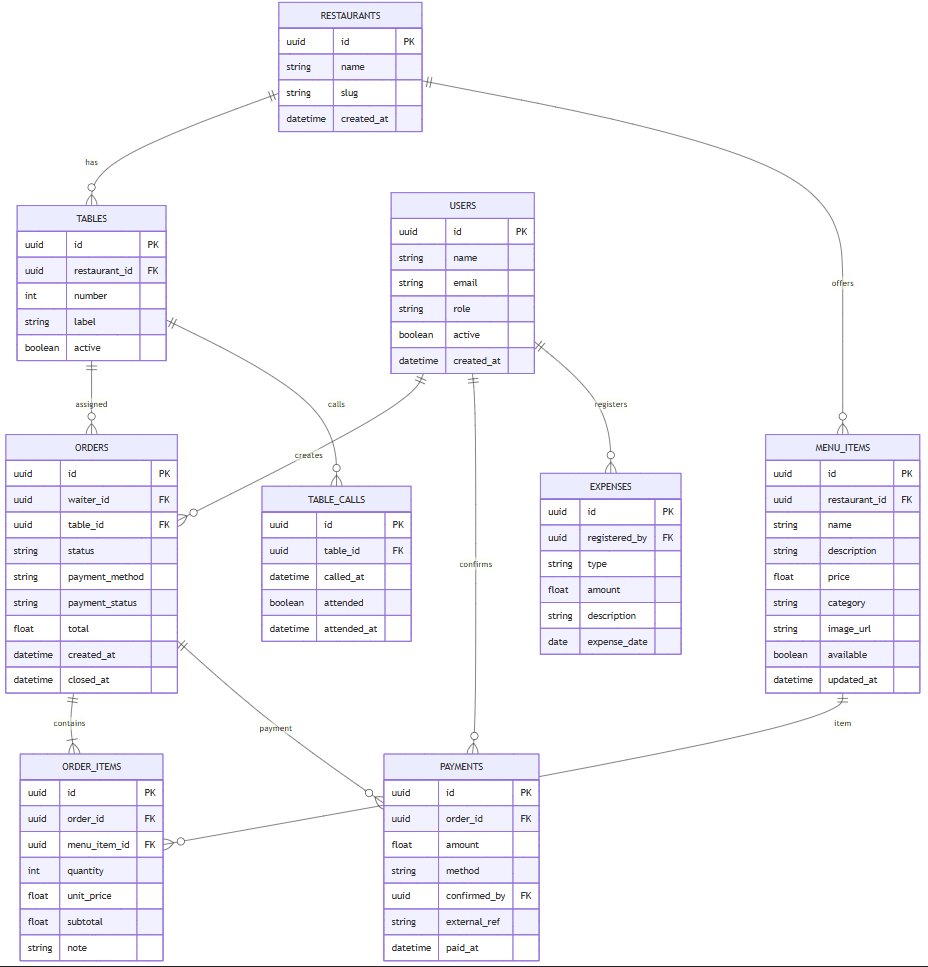
\includegraphics[width=0.95\textwidth]{img/erd_database.png}
    \caption{Modelo entidad–relación de la base de Datos}
    \label{fig:erd_database}
\end{figure}

\clearpage

\subsection{Esquema de Tablas}

A continuación se describe cada tabla del modelo de datos:

\vspace{6pt}
\noindent\textbf{\texttt{restaurants}}

\begin{tabular}{lll}
  \toprule
  \textbf{Campo} & \textbf{Tipo} & \textbf{Descripción} \\
  \midrule
  \texttt{id}         & uuid        & PK \\
  \texttt{name}       & text        & Nombre del restaurante \\
  \texttt{slug}       & text UNIQUE & Identificador en URLs públicas \\
  \texttt{created\_at} & timestamptz & Fecha de creación \\
  \bottomrule
\end{tabular}

\vspace{6pt}
\noindent\textbf{\texttt{tables}}

\begin{tabular}{lll}
  \toprule
  \textbf{Campo} & \textbf{Tipo} & \textbf{Descripción} \\
  \midrule
  \texttt{id}            & uuid    & PK \\
  \texttt{restaurant\_id} & uuid FK & Referencia a \texttt{restaurants} \\
  \texttt{number}        & integer & Número de mesa \\
  \texttt{label}         & text    & Nombre descriptivo (ej: ``Terraza 3'') \\
  \texttt{active}        & boolean & Estado activo/inactivo \\
  \bottomrule
\end{tabular}

\vspace{6pt}
\noindent\textbf{\texttt{users}}

\begin{tabular}{lll}
  \toprule
  \textbf{Campo} & \textbf{Tipo} & \textbf{Descripción} \\
  \midrule
  \texttt{id}         & uuid            & PK (sincronizado con \texttt{auth.users}) \\
  \texttt{name}       & text            & Nombre del usuario \\
  \texttt{email}      & text UNIQUE     & Correo electrónico \\
  \texttt{role}       & enum            & \texttt{waiter} | \texttt{admin} \\
  \texttt{active}     & boolean         & Estado de la cuenta \\
  \texttt{created\_at} & timestamptz    & Fecha de registro \\
  \bottomrule
\end{tabular}

\begin{notabox}
\texttt{password\_hash} se omite: Supabase Auth gestiona credenciales internamente.
El campo \texttt{role} se sincroniza hacia \texttt{auth.users.raw\_user\_meta\_data}
mediante un trigger \texttt{AFTER UPDATE}.
\end{notabox}

\vspace{6pt}
\noindent\textbf{\texttt{menu\_items}}

\begin{tabular}{lll}
  \toprule
  \textbf{Campo} & \textbf{Tipo} & \textbf{Descripción} \\
  \midrule
  \texttt{id}            & uuid          & PK \\
  \texttt{restaurant\_id} & uuid FK      & Referencia a \texttt{restaurants} \\
  \texttt{name}          & text          & Nombre del platillo \\
  \texttt{description}   & text          & Descripción \\
  \texttt{price}         & decimal(10,2) & Precio \\
  \texttt{category}      & text          & Categoría \\
  \texttt{image\_url}    & text          & URL del CDN de Storage \\
  \texttt{available}     & boolean       & Disponibilidad en tiempo real \\
  \texttt{updated\_at}   & timestamptz   & Última actualización \\
  \bottomrule
\end{tabular}

\vspace{6pt}
\noindent\textbf{\texttt{orders}}

\begin{tabular}{lll}
  \toprule
  \textbf{Campo} & \textbf{Tipo} & \textbf{Descripción} \\
  \midrule
  \texttt{id}             & uuid          & PK \\
  \texttt{waiter\_id}     & uuid FK       & Referencia a \texttt{users} \\
  \texttt{table\_id}      & uuid FK       & Referencia a \texttt{tables} \\
  \texttt{status}         & enum          & \texttt{pending | ready | delivered | cancelled} \\
  \texttt{payment\_method} & enum         & \texttt{cash | qr} \\
  \texttt{payment\_status} & enum         & \texttt{pending | confirmed} \\
  \texttt{total}          & decimal(10,2) & Total de la orden \\
  \texttt{created\_at}    & timestamptz   & Fecha de apertura \\
  \texttt{closed\_at}     & timestamptz   & Asignado automáticamente al entregar \\
  \bottomrule
\end{tabular}

\vspace{6pt}
\noindent\textbf{\texttt{order\_items}}

\begin{tabular}{lll}
  \toprule
  \textbf{Campo} & \textbf{Tipo} & \textbf{Descripción} \\
  \midrule
  \texttt{id}           & uuid          & PK \\
  \texttt{order\_id}    & uuid FK       & Referencia a \texttt{orders} \\
  \texttt{menu\_item\_id} & uuid FK     & Referencia a \texttt{menu\_items} \\
  \texttt{quantity}     & integer       & Cantidad \\
  \texttt{unit\_price}  & decimal(10,2) & Snapshot del precio al momento del pedido \\
  \texttt{subtotal}     & decimal(10,2) & Subtotal \\
  \texttt{note}         & text          & Indicación especial del cliente \\
  \bottomrule
\end{tabular}   

\vspace{6pt}
\noindent\textbf{\texttt{payments}}

\begin{tabular}{lll}
  \toprule
  \textbf{Campo} & \textbf{Tipo} & \textbf{Descripción} \\
  \midrule
  \texttt{id}           & uuid          & PK \\
  \texttt{order\_id}    & uuid FK       & Referencia a \texttt{orders} \\
  \texttt{amount}       & decimal(10,2) & Monto pagado \\
  \texttt{method}       & enum          & \texttt{cash | qr} \\
  \texttt{confirmed\_by} & uuid FK      & Admin que confirmó el pago \\
  \texttt{external\_ref} & text         & Reservado para pasarela futura \\
  \texttt{paid\_at}     & timestamptz   & Fecha/hora del pago \\
  \bottomrule
\end{tabular}

\vspace{6pt}
\noindent\textbf{\texttt{expenses}}

\begin{tabular}{lll}
  \toprule
  \textbf{Campo} & \textbf{Tipo} & \textbf{Descripción} \\
  \midrule
  \texttt{id}             & uuid          & PK \\
  \texttt{registered\_by} & uuid FK       & Usuario que registró el gasto \\
  \texttt{type}           & text          & Tipo de gasto \\
  \texttt{amount}         & decimal(10,2) & Monto \\
  \texttt{description}    & text          & Descripción \\
  \texttt{expense\_date}  & date          & Fecha del gasto \\
  \bottomrule
\end{tabular}

\clearpage
\noindent\textbf{\texttt{table\_calls}}

\begin{tabular}{lll}
  \toprule
  \textbf{Campo} & \textbf{Tipo} & \textbf{Descripción} \\
  \midrule
  \texttt{id}          & uuid        & PK \\
  \texttt{table\_id}   & uuid FK     & Referencia a \texttt{tables} \\
  \texttt{called\_at}  & timestamptz & Momento de la llamada \\
  \texttt{attended}    & boolean     & Si fue atendida \\
  \texttt{attended\_at} & timestamptz & Momento de atención \\
  \bottomrule
\end{tabular}

\section{Estructura del Proyecto}

La estructura de directorios del repositorio sigue las convenciones de Expo Router:

\begin{Verbatim}[fontsize=\small, frame=single, framesep=3mm]
gestion-comandas/
|-- app/
|   |-- (auth)/          login.tsx, _layout.tsx
|   |-- (waiter)/        tables/, orders/, _layout.tsx
|   |-- (admin)/         menu/, expenses/, reports/, _layout.tsx
|   |-- menu/[slug].tsx
|   |-- table/[slug]/[tableId].tsx
|   \-- _layout.tsx
|-- components/
|   |-- tables/TableCard.tsx
|   |-- orders/
|   |-- menu/
|   |-- customer/CallWaiterButton.tsx
|   \-- ui/
|-- lib/
|   |-- supabase.ts
|   |-- supabase-public.ts
|   |-- hooks/
|   |   |-- useOrders.ts
|   |   |-- useTables.ts
|   |   |-- useTableCalls.ts
|   |   |-- useMenu.ts
|   |   \-- useReports.ts
|   \-- types/database.types.ts
|-- supabase/
|   |-- migrations/
|   |   |-- 001_schema.sql
|   |   |-- 002_rls.sql
|   |   |-- 003_functions.sql
|   |   \-- 004_triggers.sql
|   \-- config.toml
|-- app.json
|-- eas.json
\-- tsconfig.json
\end{Verbatim}

\section{Roles y Accesos}

\begin{longtable}{p{6cm} ccc}
  \toprule
  \textbf{Funcionalidad} & \textbf{Waiter} & \textbf{Admin} & \textbf{Customer} \\
  \midrule
  \endhead
  Ver menú (solo disponibles)         & \checkmark & \checkmark & carta pública \\
  Ver menú completo (con no disp.)    & \checkmark & \checkmark & \checkmark (anónimo) \\
  Crear pedido                        & \checkmark & \checkmark & --- \\
  Actualizar estado de pedido         & \checkmark & \checkmark & --- \\
  Confirmar pago QR                   & ---        & \checkmark & --- \\
  Vista de estado de mesas            & \checkmark & --- & --- \\
  Recibir notificación de llamada     & \checkmark & --- & --- \\
  Llamar al mesero                    & ---        & --- & \checkmark \\
  Gestionar menú (CRUD + imágenes)    & ---        & \checkmark & --- \\
  Registrar gastos                    & ---        & \checkmark & --- \\
  Ver reportes financieros            & ---        & \checkmark & --- \\
  Ver ranking de platos más vendidos  & ---        & \checkmark & --- \\
  Gestionar usuarios                  & ---        & \checkmark & --- \\
  Carta digital (pública, sin auth)   & ---        & --- & --- \\
  \bottomrule
  \caption{Matriz de roles y accesos del sistema}
\end{longtable}
\chapter{Arquitectura del Sistema}

La arquitectura del sistema Gestión de Comandas adopta el modelo
\textbf{BaaS (Backend as a Service)}. En este enfoque, el cliente móvil
consume directamente los servicios proporcionados por Supabase sin la
necesidad de un backend intermedio personalizado.

Supabase provee servicios administrados de base de datos, autenticación,
almacenamiento de archivos y sincronización en tiempo real, lo cual reduce
la complejidad de infraestructura y permite enfocar el desarrollo en la
lógica de negocio y la experiencia de usuario.

\section{Diagrama de Contexto}

El diagrama de contexto muestra la interacción general entre los actores
del sistema (mesero, administrador y cliente) y los servicios principales
utilizados en la solución. Se observa cómo la aplicación móvil y la carta
digital web se comunican directamente con Supabase mediante protocolos
REST, WebSocket y mecanismos de autenticación basados en JWT.

\begin{figure}[H]
\centering
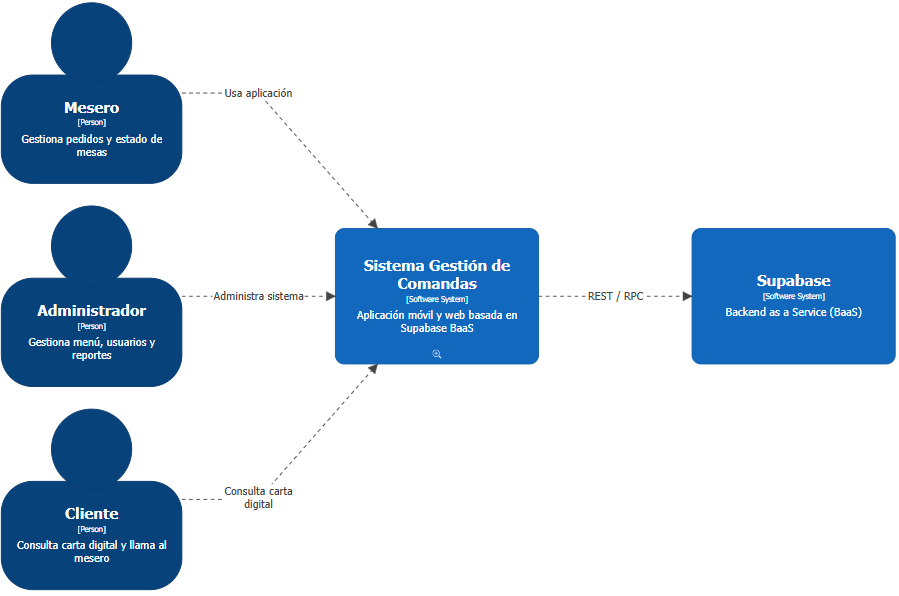
\includegraphics[width=0.95\textwidth]{img/context.png}
\caption{Diagrama de Contexto del sistema Gestión de Comandas basado en modelo BaaS}
\end{figure}

En este nivel se identifican los usuarios del sistema y los sistemas externos
con los que interactúa la solución. El cliente móvil implementado en React
Native consume directamente los servicios de Supabase PostgreSQL, Supabase
Auth, Supabase Storage y Supabase Realtime. Asimismo, la carta digital
accesible mediante navegador web permite a los clientes consultar el menú
y solicitar atención sin necesidad de autenticación tradicional.

\section{Diagrama de Contenedores}

El diagrama de contenedores describe los bloques principales que componen
la solución y cómo estos se comunican entre sí. Se distinguen claramente
los contenedores del cliente móvil, las rutas web públicas y los servicios
gestionados por Supabase.

\begin{figure}[H]
\centering
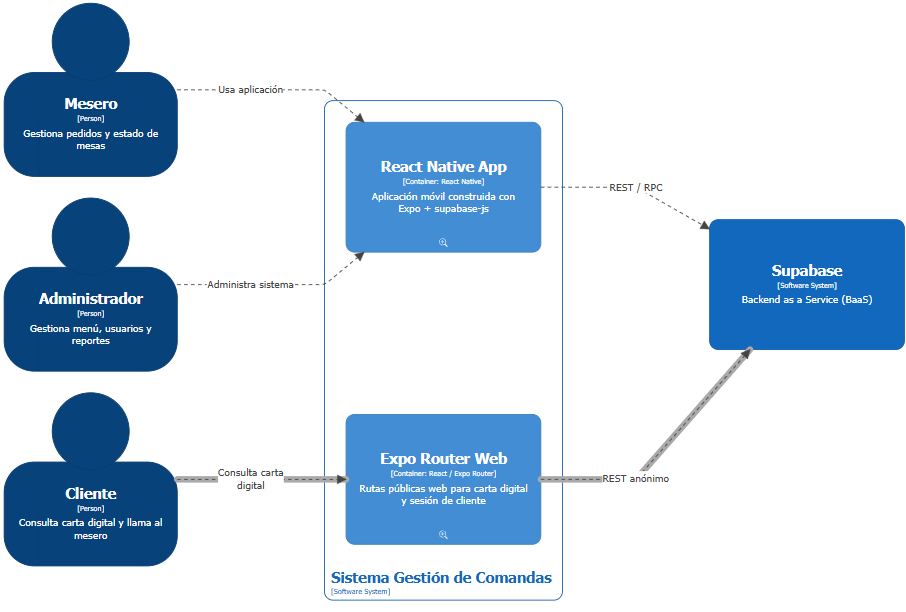
\includegraphics[width=0.95\textwidth]{img/containers.png}
\caption{Diagrama de Contenedores del sistema utilizando Supabase como Backend as a Service}
\end{figure}

La aplicación móvil desarrollada con React Native y Expo se conecta
directamente a Supabase mediante el SDK oficial supabase-js. Este cliente
permite realizar consultas a la base de datos, autenticación de usuarios,
subida de archivos y suscripción a eventos en tiempo real.

Por otro lado, Expo Router permite exponer rutas web públicas que facilitan
la visualización de la carta digital y la sesión del cliente en mesa mediante
el uso de códigos QR. Estas rutas utilizan acceso anónimo controlado mediante
las políticas de seguridad Row Level Security (RLS).

Supabase actúa como proveedor de Backend as a Service ofreciendo:

\begin{itemize}
\item Base de datos PostgreSQL con funciones SQL y políticas RLS.
\item Servicio de autenticación basado en JWT y roles.
\item Almacenamiento de imágenes del menú mediante Storage con acceso público.
\item Canales de comunicación en tiempo real mediante WebSocket.
\end{itemize}

\section{Diagrama de Componentes — Funcionalidades Clave}

\subsection{Componentes de la aplicación móvil}

El siguiente diagrama muestra los componentes principales de la aplicación
móvil utilizada por el mesero y el administrador. Estos componentes permiten
gestionar pedidos, visualizar el estado de mesas, administrar el menú y
consultar reportes financieros.

\begin{figure}[H]
\centering
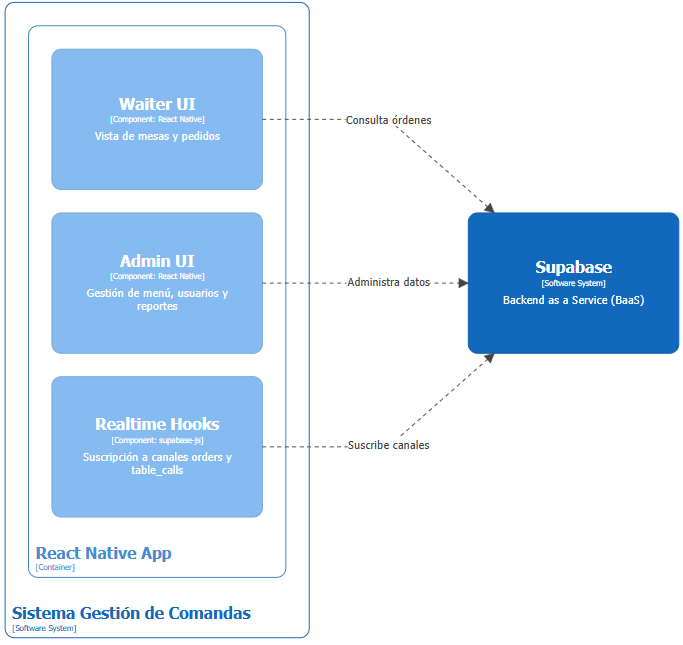
\includegraphics[width=0.95\textwidth]{img/components-mobile.png}
\caption{Componentes principales de la aplicación React Native}
\end{figure}

Los componentes Waiter UI y Admin UI representan las interfaces de usuario
según el rol autenticado. El módulo Realtime Hooks permite la suscripción a
los canales de Supabase Realtime para actualizar el estado de las mesas y
los pedidos sin necesidad de recargar la aplicación.

\subsection{Componentes de rutas web públicas}

El siguiente diagrama muestra los componentes asociados a la carta digital
y la sesión del cliente en mesa. Estas funcionalidades permiten que el cliente
visualice el menú mediante un código QR y pueda solicitar atención al mesero.

\begin{figure}[H]
\centering
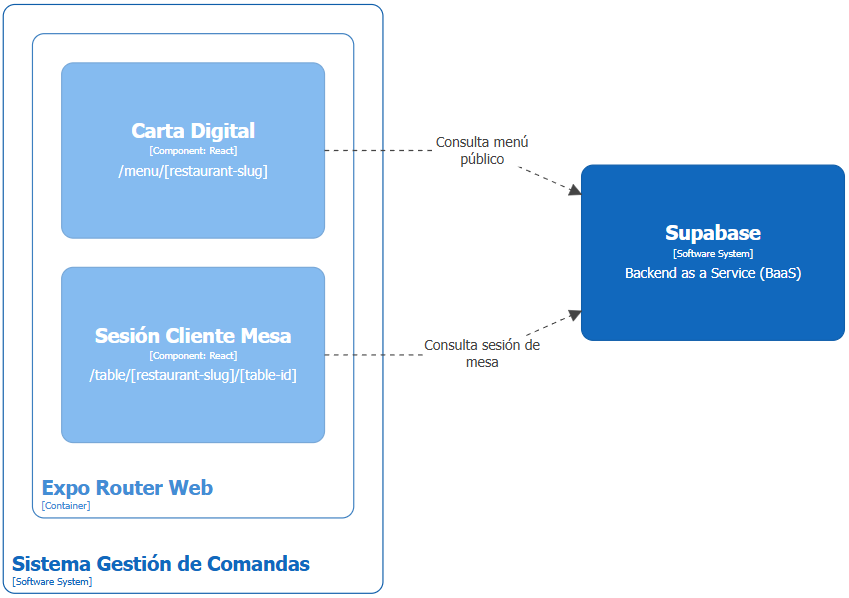
\includegraphics[width=0.95\textwidth]{img/components-web.png}
\caption{Componentes de la carta digital y sesión de cliente en mesa}
\end{figure}

Las rutas públicas permiten acceder al menú del restaurante utilizando un
identificador único (slug). La sesión de mesa permite identificar la mesa
desde la cual el cliente solicita atención, registrando eventos en la base
de datos que son posteriormente consumidos por la aplicación del mesero en
tiempo real.


\subsection{Contexto de Supabase}

El siguiente diagrama muestra cómo la aplicación cliente interactúa con los
servicios ofrecidos por Supabase dentro del modelo Backend as a Service (BaaS).
En este enfoque, el cliente móvil y las rutas web públicas consumen directamente
los servicios de autenticación, base de datos, almacenamiento y comunicación en
tiempo real sin necesidad de un backend intermedio personalizado.

\begin{figure}[H]
\centering
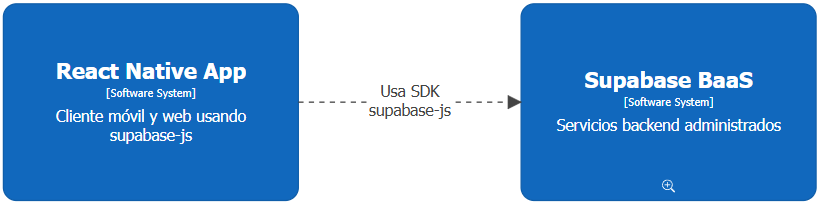
\includegraphics[width=0.9\textwidth]{img/supabase-context.png}
\caption{Relación entre la aplicación cliente y los servicios de Supabase}
\end{figure}

Supabase proporciona un conjunto de servicios integrados que permiten reducir
la complejidad de infraestructura. El SDK supabase-js facilita la conexión desde
la aplicación React Native hacia PostgreSQL, Auth, Storage y Realtime utilizando
protocolos seguros basados en JWT y WebSocket.


\subsection{Contenedores de Supabase}

El diagrama de contenedores presenta los servicios principales que conforman el
Backend as a Service utilizado en el sistema. Cada contenedor cumple una función
específica dentro de la arquitectura, permitiendo desacoplar responsabilidades
y facilitar la escalabilidad del sistema.

\begin{figure}[H]
\centering
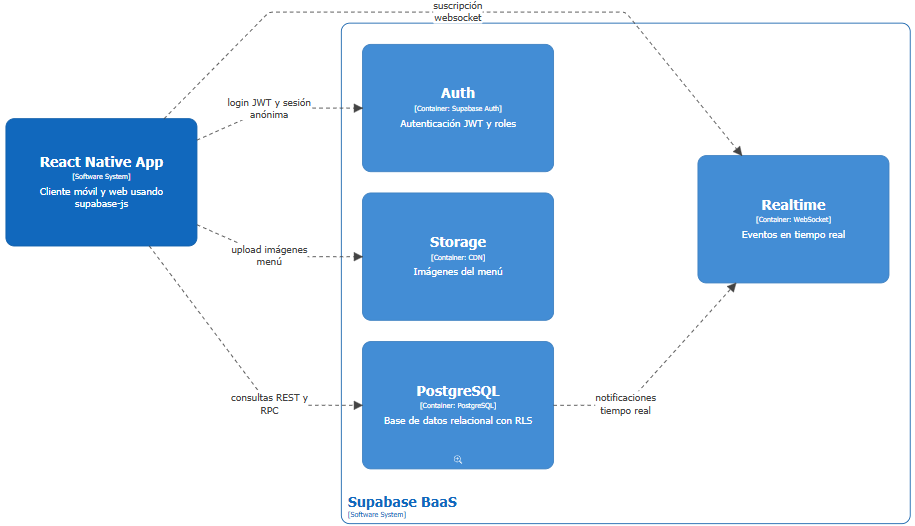
\includegraphics[width=0.9\textwidth]{img/supabase-containers.png}
\caption{Contenedores principales del entorno Supabase}
\end{figure}

El contenedor PostgreSQL almacena la información relacionada con usuarios,
mesas, pedidos, gastos y reportes. El servicio Auth permite gestionar sesiones
de usuario mediante tokens JWT, soportando autenticación tradicional y sesiones
anónimas utilizadas por la carta digital.

El servicio Storage permite almacenar imágenes de los productos del menú, las
cuales son accesibles mediante URLs públicas optimizadas mediante CDN. Por otro
lado, el servicio Realtime permite mantener sincronizados los estados de pedidos
y llamadas de clientes mediante WebSockets.


\subsection{Componentes de la Base de Datos}

El siguiente diagrama describe los componentes internos de la base de datos
implementada en Supabase. Se incluyen las tablas principales, sus relaciones
lógicas y las funciones SQL utilizadas para generar reportes financieros y
análisis de ventas.

\begin{figure}[H]
\centering
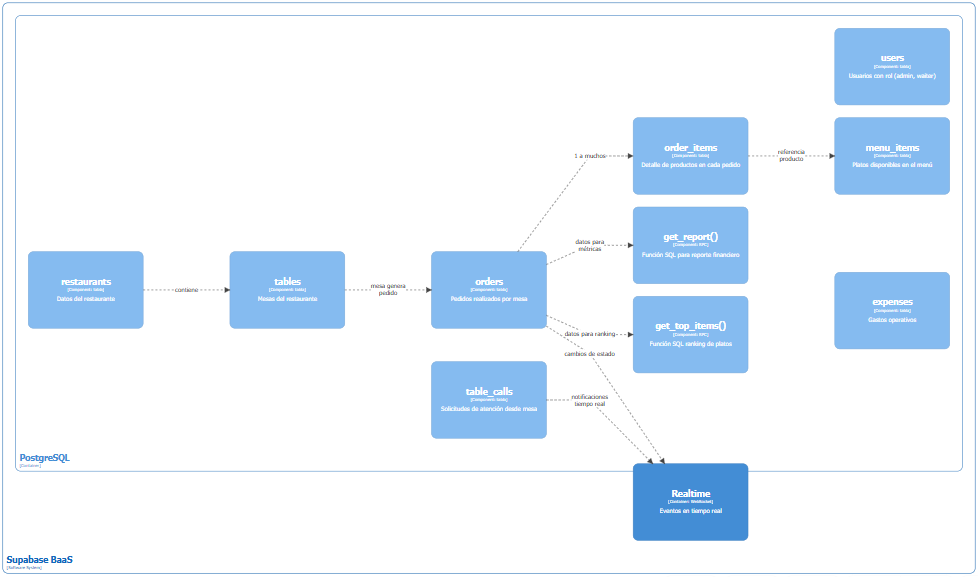
\includegraphics[width=0.95\textwidth]{img/supabase-components.png}
\caption{Componentes internos del esquema de base de datos en Supabase}
\end{figure}

La tabla \texttt{users} almacena los usuarios del sistema con sus respectivos
roles. La tabla \texttt{restaurants} permite gestionar
la información del restaurante, mientras que la tabla \texttt{tables} representa
las mesas disponibles en el establecimiento.

Las tablas \texttt{orders} y \texttt{order\_items} almacenan la información de
los pedidos realizados, manteniendo consistencia histórica de precios mediante
snapshots de los productos seleccionados. La tabla \texttt{expenses} permite
registrar los gastos operativos necesarios para el cálculo de métricas financieras.

\subsection{Vista de Estado de Mesas (Mesero)}

La pantalla principal del mesero muestra en tiempo real el estado de cada
mesa asignada. Esta funcionalidad se basa en la suscripción al canal
\texttt{orders} de Supabase Realtime, permitiendo actualizar los estados
de los pedidos sin necesidad de recargar la aplicación.

Adicionalmente, la aplicación escucha el canal \texttt{table\_calls}, el cual
permite detectar cuando un cliente solicita atención desde su mesa mediante
la carta digital.

\begin{center}
\begin{tabular}{ll}
  \toprule
  \textbf{Estado visual} & \textbf{Condición en DB} \\
  \midrule
  Libre                  & Sin orden activa para esa mesa en la fecha actual \\
  Pendiente              & \texttt{status = 'pending'} \\
  Listo para entregar    & \texttt{status = 'ready'} \\
  Entregado              & \texttt{status = 'delivered'} \\
  Cliente llama          & Registro en \texttt{table\_calls} con \texttt{attended = false} \\
  \bottomrule
\end{tabular}
\end{center}

Este mecanismo permite mantener sincronizados los estados entre múltiples
dispositivos conectados simultáneamente, asegurando consistencia en la
información mostrada al personal del restaurante.
\chapter{Metodología Aplicada}

% ── 5.1 ──────────────────────────────────────────────────
\section{Metodología de Desarrollo}

Para el desarrollo del proyecto se adoptó la metodología ágil \textbf{Scrum},
dado que permite una alta flexibilidad y adaptación a los cambios, además de
fomentar una comunicación constante entre los miembros del equipo. Scrum se
basa en ciclos de trabajo cortos y entregables funcionales (sprints) que
permiten un seguimiento continuo del progreso.

El proceso de desarrollo sigue las siguientes fases dentro del marco de Scrum:

\begin{itemize}[leftmargin=1.5em]
  \item \textbf{Product Backlog:} Lista priorizada de los requisitos del
        proyecto, mantenida y priorizada por el Product Owner.
  \item \textbf{Sprint Planning:} Antes de cada sprint el equipo selecciona
        los ítems del backlog a completar y se compromete a entregarlos.
  \item \textbf{Daily Stand-Up:} Reuniones diarias breves para revisar
        progreso, detectar bloqueos y ajustar tareas.
  \item \textbf{Sprint Review:} Al final del sprint se presenta el incremento
        al Product Owner y partes interesadas.
  \item \textbf{Sprint Retrospective:} El equipo identifica áreas de mejora
        en el proceso y aplica ajustes al siguiente sprint.
\end{itemize}

\section{Ciclo de Vida del Proyecto}

El proyecto se organizó en \textbf{3 sprints de 4 semanas} cada uno:

\begin{longtable}{>{\bfseries}p{1.5cm} p{11.5cm}}
  \toprule
  \textbf{Sprint} & \textbf{Alcance} \\
  \midrule
  \endhead

  1 & Configuración del proyecto, diseño del schema en Supabase,
      autenticación, RLS, CRUD del menú e integración con Storage
      para manejo de imágenes. \\[4pt]

  2 & Registro de pedidos, vista de mesas en tiempo real mediante
      Realtime, manejo de estados de pedido, módulo de gastos,
      funciones SQL de reportes y ranking de platos. \\[4pt]

  3 & Carta digital pública por QR, sesión anónima por mesa,
      llamada al mesero, confirmación de pagos por admin,
      pruebas finales y despliegue con EAS Build. \\

  \bottomrule
  \caption{Release Plan — Sprints del proyecto}
\end{longtable}

\section{Herramientas de Gestión}

\begin{itemize}[leftmargin=1.5em]
  \item \textbf{Notion:} Gestión del sprint backlog con vista Kanban
        (Por hacer / En progreso / En revisión / Completado),
        centralización de documentación técnica y seguimiento de tareas.
  \item \textbf{GitHub:} Control de versiones distribuido, revisión de código
        mediante pull requests y entrega de incrementos de forma controlada.
  \item \textbf{Discord:} Canal principal de comunicación cotidiana,
        dividido en espacios temáticos (desarrollo, diseño, pruebas).
  \item \textbf{Excalidraw:} Diagramación colaborativa de esquemas de base de
        datos, flujos de navegación y arquitectura del sistema.
  \item \textbf{Postman:} Testing y documentación de llamadas RPC y REST
        durante el desarrollo e integración.
\end{itemize}
\chapter{Seguimiento y Desarrollo Grupal}

\section{Planificación del Trabajo}

\subsection*{Sprint 1 — Fundación: base de datos, autenticación y roles}

\textbf{Objetivo:}  
Setup del proyecto, schema de BD, autenticación, RLS y CRUD del menú.

\textbf{Historias de Usuario}

\begin{itemize}[leftmargin=1.5em]

\item \textbf{Setup e infraestructura}

\begin{itemize}
\item HU-01: Inicializar proyecto Expo con TypeScript y Expo Router
\item HU-02: Configurar proyecto Supabase y variables de entorno
\item HU-03: Crear migración de esquema inicial de la base de datos
\item HU-04: Crear constraint de orden activa única por mesa
\item HU-05: Crear trigger set\_closed\_at al entregar una orden
\end{itemize}

\item \textbf{Autenticación y roles}

\begin{itemize}
\item HU-06: Implementar pantalla de login para mesero y admin
\item HU-07: Proteger rutas según rol con guards de navegación
\item HU-08: Crear trigger sync\_role\_to\_auth para sincronizar rol
\item HU-09: Implementar cierre de sesión
\end{itemize}

\item \textbf{Row Level Security}

\begin{itemize}
\item HU-10: Implementar RLS para la tabla orders
\item HU-11: Implementar RLS para expenses, menu\_items y table\_calls
\end{itemize}

\item \textbf{Gestión de usuarios (admin)}

\begin{itemize}
\item HU-12: Listar usuarios del sistema (admin)
\item HU-13: Crear nuevo usuario mesero o admin (admin)
\item HU-14: Activar y desactivar usuario (admin)
\end{itemize}

\item \textbf{Gestión de mesas (admin)}

\begin{itemize}
\item HU-15: CRUD de mesas del restaurante (admin)
\item HU-16: Gestionar restaurante y su slug (admin)
\end{itemize}

\end{itemize}


\subsection*{Sprint 2 — Operación: menú, pedidos, pagos y gastos}

\textbf{Objetivo:}  
Registro de pedidos, vista de mesas en tiempo real y módulo financiero.

\textbf{Historias de Usuario}

\begin{itemize}[leftmargin=1.5em]

\item \textbf{Gestión de menú (admin)}

\begin{itemize}
\item HU-17: Listar ítems del menú con filtro por categoría (admin)
\item HU-18: Crear ítem del menú con imagen (admin)
\item HU-19: Editar precio y descripción de un ítem (admin)
\item HU-20: Activar o desactivar disponibilidad de un ítem (admin)
\item HU-21: Eliminar ítem del menú (admin)
\end{itemize}

\item \textbf{Toma de pedidos (mesero)}

\begin{itemize}
\item HU-22: Ver el menú disponible al tomar un pedido (mesero)
\item HU-23: Crear una nueva orden seleccionando mesa e ítems (mesero)
\item HU-24: Ver detalle de una orden activa (mesero)
\item HU-25: Agregar ítems a una orden existente (mesero)
\item HU-26: Marcar una orden como entregada (mesero)
\item HU-27: Cancelar una orden (mesero y admin)
\item HU-28: Seleccionar método de pago al crear la orden (mesero)
\end{itemize}

\item \textbf{Pagos (admin)}

\begin{itemize}
\item HU-29: Ver órdenes con pago QR pendiente de confirmación (admin)
\item HU-30: Confirmar pago QR de una orden (admin)
\item HU-31: Mostrar QR estático de pago al cliente (mesero)
\end{itemize}

\item \textbf{Gastos operativos (admin)}

\begin{itemize}
\item HU-32: Registrar un gasto operativo (admin)
\item HU-33: Listar gastos por rango de fechas (admin)
\item HU-34: Editar y eliminar un gasto (admin)
\end{itemize}

\end{itemize}


\subsection*{Sprint 3 — Tiempo real, carta digital y reportes}

\textbf{Objetivo:}  
Carta digital pública, sesión de cliente en mesa, pagos y despliegue final.

\textbf{Historias de Usuario}

\begin{itemize}[leftmargin=1.5em]

\item \textbf{Vista de mesas en tiempo real (mesero)}

\begin{itemize}
\item HU-35: Ver estado de todas las mesas asignadas (mesero)
\item HU-36: Actualizar estado de mesas en tiempo real sin recargar (mesero)
\item HU-37: Recibir notificación cuando un pedido está listo (mesero)
\item HU-38: Manejar reconexión automática del canal Realtime (mesero)
\end{itemize}

\item \textbf{Llamada al mesero (cliente → mesero)}

\begin{itemize}
\item HU-39: Mostrar botón "Llamar al mesero" en la sesión de cliente en mesa
\item HU-40: Recibir notificación de llamada de cliente en tiempo real (mesero)
\item HU-41: Marcar llamada de cliente como atendida (mesero)
\end{itemize}

\item \textbf{Carta digital pública (web)}

\begin{itemize}
\item HU-42: Publicar carta digital accesible por URL sin login
\item HU-43: Mostrar carta organizada por categorías con imágenes y precios
\item HU-44: Generar y mostrar QR del restaurante para carta pública (admin)
\end{itemize}

\item \textbf{Sesión de cliente en mesa (web)}

\begin{itemize}
\item HU-45: Iniciar sesión anónima al escanear el QR de la mesa
\item HU-46: Ver menú completo (incluyendo no disponibles) desde la sesión de mesa
\item HU-47: Generar QR individual por mesa (admin)
\end{itemize}

\item \textbf{Reportes financieros (admin)}

\begin{itemize}
\item HU-48: Crear función SQL get\_report para ingresos y egresos
\item HU-49: Crear función SQL get\_top\_items para ranking de platos
\item HU-50: Pantalla de reporte financiero por período (admin)
\item HU-51: Pantalla de ranking de platos más vendidos (admin)
\end{itemize}

\end{itemize}

\bigskip
\begin{center}
\textit{51 historias de usuario · 3 sprints · 6 semanas}
\end{center}


\section{Roles y Responsabilidades}

\begin{center}
\begin{tabular}{ll}
  \toprule
  \textbf{Integrante} & \textbf{Rol} \\
  \midrule
  Acebey Zalazar Jimmy Randall & Desarrollador \\
  Cáceres Véliz Erick Alvaro   & Desarrollador \\
  Revollo Bernal Amilcar Diego & Scrum Master \\
  Siles Espicho Adrian Eloy    & Desarrollador  \\
  Tinta Mamani Jairo Amado     & Desarrollador \\
  \bottomrule
\end{tabular}
\end{center}


\section{Control de Versiones}

El proyecto utiliza un sistema de control de versiones distribuido con
\textbf{Git}, gestionado en un único repositorio alojado en GitHub
(\texttt{gestion-comandas}). Este enfoque centralizado permite una
coordinación eficiente entre el desarrollo del frontend móvil, las rutas
web públicas y las migraciones de base de datos.

La estrategia de ramas adoptada es:

\begin{itemize}[leftmargin=1.5em]
  \item \textbf{\texttt{main}:} rama de producción; solo recibe merges mediante Pull Requests aprobados.
  \item \textbf{\texttt{feature/[nombre]}:} una rama por historia de usuario o tarea de sprint.
\end{itemize}


\section{Reporte de Avances}

\subsection{Indicadores de Progreso}

\begin{longtable}{>{\bfseries}p{2cm} p{9cm} c}
  \toprule
  \textbf{ID} & \textbf{Historia de Usuario} & \textbf{Completada} \\
  \midrule
  \endhead

  HU-01 & Inicializar proyecto Expo con TypeScript y Expo Router & \checkmark \\
  HU-02 & Configurar proyecto Supabase y variables de entorno & \checkmark \\
  HU-03 & Crear migración de esquema inicial de la base de datos & \checkmark \\
  HU-04 & Crear constraint de orden activa única por mesa & \checkmark \\
  HU-05 & Crear trigger set\_closed\_at al entregar una orden & \checkmark \\
  HU-06 & Implementar pantalla de login para mesero y admin & \checkmark \\
  HU-07 & Proteger rutas según rol con guards de navegación & \checkmark \\
  HU-08 & Crear trigger sync\_role\_to\_auth para sincronizar rol & \checkmark \\
  HU-09 & Implementar cierre de sesión & \checkmark \\
  HU-10 & Implementar RLS para la tabla orders & \checkmark \\
  HU-11 & Implementar RLS para expenses, menu\_items y table\_calls & \checkmark \\
  HU-12 & Listar usuarios del sistema (admin) & \checkmark \\
  HU-13 & Crear nuevo usuario mesero o admin (admin) & \checkmark \\
  HU-14 & Activar y desactivar usuario (admin) & \checkmark \\
  HU-15 & CRUD de mesas del restaurante (admin) & \checkmark \\
  HU-16 & Gestionar restaurante y su slug (admin) & \checkmark \\
  HU-17 & Listar ítems del menú con filtro por categoría (admin) & \checkmark \\
  HU-18 & Crear ítem del menú con imagen (admin) & \checkmark \\
  HU-19 & Editar precio y descripción de un ítem (admin) & \checkmark \\
  HU-20 & Activar o desactivar disponibilidad de un ítem (admin) & \checkmark \\
  HU-21 & Eliminar ítem del menú (admin) & \checkmark \\
  HU-22 & Ver el menú disponible al tomar un pedido (mesero) & \checkmark \\
  HU-23 & Crear una nueva orden seleccionando mesa e ítems (mesero) & \checkmark \\
  HU-24 & Ver detalle de una orden activa (mesero) & \checkmark \\
  HU-25 & Agregar ítems a una orden existente (mesero) & \checkmark \\
  HU-26 & Marcar una orden como entregada (mesero) & \checkmark \\
  HU-27 & Cancelar una orden (mesero y admin) & \checkmark \\
  HU-28 & Seleccionar método de pago al crear la orden (mesero) & \checkmark \\
  HU-29 & Ver órdenes con pago QR pendiente de confirmación (admin) & \checkmark \\
  HU-30 & Confirmar pago QR de una orden (admin) & \checkmark \\
  HU-31 & Mostrar QR estático de pago al cliente (mesero) & \checkmark \\
  HU-32 & Registrar un gasto operativo (admin) & \checkmark \\
  HU-33 & Listar gastos por rango de fechas (admin) & \checkmark \\
  HU-34 & Editar y eliminar un gasto (admin) & \checkmark \\
  HU-35 & Ver estado de todas las mesas asignadas (mesero) & \checkmark \\
  HU-36 & Actualizar estado de mesas en tiempo real sin recargar (mesero) & \checkmark \\
  HU-37 & Recibir notificación cuando un pedido está listo (mesero) & \checkmark \\
  HU-38 & Manejar reconexión automática del canal Realtime (mesero) & \checkmark \\
  HU-39 & Mostrar botón "Llamar al mesero" en la sesión de cliente en mesa & \checkmark \\
  HU-40 & Recibir notificación de llamada de cliente en tiempo real (mesero) & \checkmark \\
  HU-41 & Marcar llamada de cliente como atendida (mesero) & \checkmark \\
  HU-42 & Publicar carta digital accesible por URL sin login & \checkmark \\
  HU-43 & Mostrar carta organizada por categorías con imágenes y precios & \checkmark \\
  HU-44 & Generar y mostrar QR del restaurante para carta pública (admin) & \checkmark \\
  HU-45 & Iniciar sesión anónima al escanear el QR de la mesa & \checkmark \\
  HU-46 & Ver menú completo (incluyendo no disponibles) desde la sesión de mesa & \checkmark \\
  HU-47 & Generar QR individual por mesa (admin) & \checkmark \\
  HU-48 & Crear función SQL get\_report para ingresos y egresos & \checkmark \\
  HU-49 & Crear función SQL get\_top\_items para ranking de platos & \checkmark \\
  HU-50 & Pantalla de reporte financiero por período (admin) & \checkmark \\
  HU-51 & Pantalla de ranking de platos más vendidos (admin) & \checkmark \\

  \bottomrule
  \caption{Indicadores de progreso por historia de usuario}
\end{longtable}

\subsection{Dificultades Encontradas}

\begin{itemize}[leftmargin=1.5em]

\item \textbf{Pausa automática del free tier de Supabase:}
La base de datos se pausa tras períodos de inactividad,
por lo que se implementó un ping periódico para mantener
activo el servicio durante el desarrollo.

\item \textbf{Reconexión de canales Realtime:}
Las conexiones móviles inestables pueden interrumpir la
sincronización en tiempo real. Se implementó manejo de
eventos \texttt{CHANNEL\_ERROR} y \texttt{TIMED\_OUT}
con reintento automático.

\item \textbf{Persistencia de precios históricos:}
Para mantener la consistencia financiera, el precio del
producto se almacena como snapshot en el momento del pedido,
evitando inconsistencias cuando el admin modifica el menú.

\end{itemize}


\section{Comunicación}

El equipo empleó las siguientes herramientas de comunicación y colaboración:

\begin{itemize}[leftmargin=1.5em]
  \item \textbf{Notion:} planificación de tareas, backlog y documentación técnica.
  \item \textbf{GitHub:} control de versiones y revisión de código mediante pull requests.
  \item \textbf{Discord:} canal principal de comunicación durante el desarrollo.
  \item \textbf{WhatsApp:} coordinación rápida para decisiones puntuales.
\end{itemize}
% ============================================================
%  07_pruebas.tex
% ============================================================
\chapter{Pruebas y Resultados}

% ── 7.1 ──────────────────────────────────────────────────
\section{Plan de Pruebas}

Se efectuaron evaluaciones funcionales, de usabilidad y de integración con el
propósito de verificar el cumplimiento de los requisitos, analizar la facilidad de
uso y garantizar la estabilidad del sistema en condiciones reales de operación.

\subsection{Tipos de Pruebas Aplicadas}

\begin{itemize}[leftmargin=1.5em]
  \item \textbf{Pruebas funcionales:} Verificación de que cada módulo responde
        conforme a los requisitos funcionales (RF-01 a RF-12).
  \item \textbf{Pruebas de navegación:} Análisis de la coherencia de los flujos
        de pantalla, menús y transiciones entre roles.
  \item \textbf{Pruebas de integración:} Validación de la comunicación entre
        el cliente React Native y los servicios de Supabase (REST, RPC,
        Realtime, Storage).
  \item \textbf{Pruebas Realtime:} Verificación de la latencia de notificaciones
        en el canal \texttt{orders} y \texttt{table\_calls} bajo condiciones de
        red móvil.
  \item \textbf{Pruebas de seguridad / RLS:} Intentos de acceso cruzado entre
        roles para validar que las políticas RLS bloqueen correctamente.
  \item \textbf{Pruebas exploratorias:} Recorrido libre de la aplicación por
        evaluadores externos para detectar comportamientos inesperados.
  \item \textbf{Pruebas de UX/UI:} Evaluación de la experiencia del usuario,
        priorizando interfaces simples y claras.
\end{itemize}

\subsection{Escenarios Evaluados}

\begin{enumerate}[leftmargin=1.8em]
  \item Registro y login de mesero y administrador.
  \item Creación de un pedido con selección de platillos, mesa y método de pago.
  \item Actualización del estado de un pedido (\texttt{pending} → \texttt{ready}
        → \texttt{delivered}) y verificación de notificación en tiempo real.
  \item Vista de estado de mesas: validar que los cambios de estado aparecen
        sin recargar la pantalla.
  \item Llamada al mesero desde la sesión de cliente en mesa y recepción de
        notificación en el dispositivo del mesero.
  \item Acceso a la carta digital pública (sin login) y validación de que solo
        aparecen ítems con \texttt{available = true}.
  \item Gestión del menú por el admin: crear, editar precio, cambiar disponibilidad,
        subir imagen.
  \item Registro de gastos operativos y generación de reporte financiero por rango
        de fechas.
  \item Consulta del ranking de platos más vendidos (RPC \texttt{get\_top\_items}).
  \item Confirmación de pago QR por el admin y verificación de contabilización
        en el reporte.
  \item Intento de acceso cruzado: mesero intentando acceder a reportes
        (debe ser bloqueado por RLS).
  \item Simulación de pérdida de conexión y reconexión automática del canal
        Realtime.
\end{enumerate}

\subsection{Herramientas de Soporte}

\begin{itemize}[leftmargin=1.5em]
  \item \textbf{Emuladores Android (Android Studio):} Pruebas preliminares de
        compatibilidad y funcionalidad básica.
  \item \textbf{Dispositivos físicos Android:} Validaciones de rendimiento y
        experiencia real del usuario final.
  \item \textbf{Expo Go / EAS Build:} Distribución de builds de prueba al equipo.
  \item \textbf{Supabase Dashboard:} Inspección directa de la base de datos y
        logs de RLS para verificar políticas.
  \item \textbf{Postman:} Pruebas directas de funciones RPC y endpoints REST.
\end{itemize}

\subsection{Condiciones de Aprobación}

Una prueba se considera superada cuando:
\begin{itemize}[leftmargin=1.5em]
  \item Las funcionalidades operan conforme a los requisitos funcionales
        y criterios de aceptación definidos.
  \item Las políticas RLS bloquean accesos no autorizados sin excepción.
  \item Las notificaciones Realtime llegan en menos de 2 segundos en red WiFi.
  \item La experiencia del usuario es valorada como satisfactoria.
  \item No se detectan fallos críticos en las pruebas exploratorias.
\end{itemize}

% ── 7.2 ──────────────────────────────────────────────────
\section{Resultados Obtenidos}

\subsection{Registro y Gestión de Pedidos}

El flujo de creación de pedidos fue validado exitosamente en dispositivos físicos.
El mesero puede seleccionar platillos del menú, asignar una mesa y elegir el método
de pago. El cálculo del total se realiza automáticamente al agregar ítems.

\subsection{Vista de Mesas en Tiempo Real}

La pantalla de estado de mesas del mesero actualizó correctamente los estados
(\texttt{pending}, \texttt{ready}, \texttt{delivered}) al recibir eventos del canal
\texttt{orders} de Supabase Realtime, sin necesidad de recargar la pantalla. La
latencia promedio observada fue inferior a 1.5 segundos en red WiFi.

\subsection{Carta Digital y Sesión de Cliente}

La carta digital pública fue accedida correctamente desde navegadores móviles
sin descarga de app. La sesión anónima por mesa se inició correctamente al
escanear el QR de mesa y el cliente pudo llamar al mesero, recibiendo el mesero
la notificación en tiempo real vía canal \texttt{table\_calls}.

\subsection{Reportes Financieros}

Las funciones RPC \texttt{get\_report} y \texttt{get\_top\_items} devolvieron
resultados correctos en todas las combinaciones de rango de fechas probadas.
La validación de rol dentro de la función \texttt{get\_report} bloqueó
correctamente el acceso cuando se intentó invocar con un token de rol
\texttt{waiter}.

\subsection{Seguridad RLS}

Todos los intentos de acceso cruzado entre roles fueron bloqueados por las
políticas RLS. El mesero no pudo leer órdenes de otros meseros ni acceder
a la tabla \texttt{expenses}. El cliente anónimo solo pudo insertar en
\texttt{table\_calls} para su propia mesa.

% ── 7.3 ──────────────────────────────────────────────────
\section{Limitaciones Conocidas}

\subsection{Free Tier de Supabase}

\begin{center}
\begin{tabular}{ll}
  \toprule
  \textbf{Límite} & \textbf{Valor} \\
  \midrule
  Base de datos                      & 500 MB \\
  Storage                            & 1 GB \\
  Requests mensuales                 & 50,000 \\
  Conexiones Realtime simultáneas    & 200 \\
  Inactividad (pausa automática)     & 7 días sin actividad \\
  \bottomrule
\end{tabular}
\end{center}

\begin{alertbox}
La pausa automática por inactividad es un riesgo operacional real en producción.
Debe resolverse mediante un ping periódico (ej. \texttt{cron-job.org}) o migración
al tier Pro (\$25/mes) antes del primer despliegue en un restaurante real.
\end{alertbox}

\subsection{Limitaciones de Alcance Documentadas}

\begin{itemize}[leftmargin=1.5em]
  \item La \textbf{reasignación de órdenes} entre meseros no está soportada
        en tiempo real. Si el admin reasigna una orden, el nuevo mesero no
        recibe el evento Realtime hasta el próximo ciclo de polling.
  \item El \textbf{cliente en mesa no puede crear órdenes directamente}.
        Requeriría un estado \texttt{draft} y un flujo de confirmación por
        el mesero, fuera del alcance actual.
  \item El \textbf{pago QR es estático} y su verificación es manual por el
        admin. No hay integración con pasarelas de pago en este alcance.
  \item Las \textbf{cancelaciones parciales y devoluciones} no tienen flujo
        dedicado. Se recomienda implementar en versiones posteriores.
\end{itemize}

% ── 7.4 ──────────────────────────────────────────────────
\section{Mejoras Propuestas}

\begin{enumerate}[leftmargin=1.8em]
  \item \textbf{Pasarela de pagos:} Integrar con una pasarela (ej. Mercado Pago
        o Stripe) para verificar pagos QR de forma automática.
  \item \textbf{Dashboard live global:} Implementar una vista de operación en
        tiempo real para el admin con estado de todas las mesas y meseros
        (descartada del alcance actual por complejidad).
  \item \textbf{Cancelaciones parciales:} Añadir flujo para devolver o cancelar
        ítems individuales de una orden sin cancelar toda la comanda.
  \item \textbf{Reasignación de órdenes en tiempo real:} Soporte completo de
        Realtime al reasignar una orden a otro mesero.
  \item \textbf{Soporte multi-idioma:} Internacionalización de la interfaz
        para restaurantes con clientes internacionales.
  \item \textbf{Modo offline básico:} Caché local de las órdenes activas para
        operar sin conexión y sincronizar al reconectar.
\end{enumerate}
% ============================================================
%  08_conclusiones.tex
% ============================================================
\chapter{Conclusiones}

El desarrollo del proyecto \textbf{Gestión de Comandas} representa un esfuerzo
exitoso que logró cumplir con los objetivos planteados, consolidando una plataforma
integral para la modernización operativa de restaurantes pequeños y medianos. La
aplicación implementa funcionalidades clave como el registro de pedidos en tiempo
real, la vista de estado de mesas vía Supabase Realtime, la gestión diferenciada por
roles con Row Level Security, los reportes financieros calculados server-side mediante
funciones PostgreSQL, y la carta digital pública accesible sin app desde cualquier
dispositivo.

Este logro fue posible gracias a la adopción del modelo BaaS con Supabase, que
permitió eliminar la necesidad de un backend intermedio propio, reduciendo la
complejidad operacional y el costo de infraestructura. La elección de React Native
con Expo garantiza actualizaciones OTA sin pasar por las tiendas de aplicaciones,
lo que es especialmente valioso en un entorno de restaurante donde la continuidad
del servicio es crítica.

El trabajo en equipo bajo la metodología \textbf{Scrum} demostró ser fundamental
para el progreso organizado del proyecto, permitiendo una distribución efectiva de
responsabilidades y una supervisión constante del avance a través de sprints bien
definidos. La asignación clara de roles, combinada con el uso estratégico de
herramientas colaborativas como GitHub, Notion y Discord, facilitó la resolución
de desafíos técnicos y aseguró la entrega de incrementos funcionales en cada
iteración.

Si bien la plataforma alcanzó sus objetivos principales, algunas funcionalidades
avanzadas, como la integración con pasarelas de pago, el dashboard live global
para el administrador y las cancelaciones parciales, representan oportunidades de
mejora para futuras iteraciones que podrán construirse sobre la base tecnológica
y funcional sólida establecida en este desarrollo.

% ── 8.1 ──────────────────────────────────────────────────
\section{Recomendaciones}

\subsection{Futuros Desarrollos}

\begin{itemize}[leftmargin=1.5em]
  \item \textbf{Integración con pasarelas de pago:} Conectar con Mercado Pago,
        Stripe u otra pasarela disponible en el mercado local para automatizar
        la verificación de pagos QR y eliminar la confirmación manual.
  \item \textbf{Dashboard live global:} Implementar la vista global de operación
        del restaurante para el admin, mostrando el estado de todas las mesas
        y meseros en tiempo real.
  \item \textbf{Cancelaciones parciales y devoluciones:} Añadir un flujo
        dedicado para devolver o cancelar ítems individuales dentro de una orden.
  \item \textbf{Modo offline básico:} Implementar caché local de órdenes activas
        para operar sin conexión y sincronizar al reconectar, usando tecnologías
        como MMKV o SQLite en el cliente React Native.
  \item \textbf{Soporte multi-sucursal avanzado:} La tabla \texttt{restaurants}
        ya habilita multi-sucursal; la siguiente iteración puede añadir un panel
        de administración por cadena de restaurantes.
\end{itemize}

\subsection{Optimizaciones Técnicas}

\begin{itemize}[leftmargin=1.5em]
  \item \textbf{Migración al tier Pro de Supabase:} Eliminar el riesgo de pausa
        automática por inactividad antes del despliegue en producción real.
  \item \textbf{Índices adicionales:} Añadir índices compuestos en
        \texttt{orders(waiter\_id, status)} y
        \texttt{order\_items(order\_id, menu\_item\_id)} para optimizar
        las consultas más frecuentes en horas pico.
  \item \textbf{Pruebas automatizadas:} Incorporar pipelines de CI/CD con suites
        de testing unitario (Jest), integración y end-to-end (Detox) para reducir
        la deuda de regresión.
  \item \textbf{Monitoreo de rendimiento:} Integrar Sentry o similar para
        captura de errores y métricas de rendimiento en producción.
\end{itemize}

\subsection{Gestión y Comunicación}

\begin{itemize}[leftmargin=1.5em]
  \item \textbf{Documentación técnica continua:} Establecer un proceso sistemático
        para mantener actualizados el esquema de BD, las políticas RLS y las
        decisiones de arquitectura en el repositorio.
  \item \textbf{Protocolos de code review:} Definir checklists estandarizados
        para revisiones de código que aseguren calidad y consistencia.
  \item \textbf{Capacitación en herramientas:} Realizar sesiones de entrenamiento
        en el uso avanzado de Supabase (migraciones, funciones RPC, Realtime)
        para todo el equipo de desarrollo.
\end{itemize}
% ============================================================
%  09_bibliografia.tex
% ============================================================
\chapter{Bibliografía}

\section{Tecnologías y Frameworks}

\begin{itemize}[leftmargin=1.5em]
  \item Supabase. (s/f). \textit{Supabase Documentation}.
        Recuperado el 11 de noviembre de 2025, de
        \url{https://supabase.com/docs}

  \item Supabase. (s/f). \textit{supabase-js v2 Reference}.
        Recuperado el 11 de noviembre de 2025, de
        \url{https://supabase.com/docs/reference/javascript}

  \item Supabase. (s/f). \textit{Anonymous Sign-ins}.
        Recuperado el 11 de noviembre de 2025, de
        \url{https://supabase.com/docs/guides/auth/anonymous-sign-ins}

  \item Expo. (s/f). \textit{Expo Documentation}.
        Recuperado el 11 de noviembre de 2025, de
        \url{https://docs.expo.dev/}

  \item Expo. (s/f). \textit{Expo Router — Web Support}.
        Recuperado el 11 de noviembre de 2025, de
        \url{https://docs.expo.dev/router/introduction/}

  \item Expo. (s/f). \textit{EAS Build}.
        Recuperado el 11 de noviembre de 2025, de
        \url{https://docs.expo.dev/build/introduction/}

  \item React Native. (s/f). \textit{React Native Documentation}.
        Recuperado el 11 de noviembre de 2025, de
        \url{https://reactnative.dev/docs/getting-started}

  \item PostgreSQL Global Development Group. (s/f).
        \textit{PostgreSQL Row Level Security}.
        Recuperado el 11 de noviembre de 2025, de
        \url{https://www.postgresql.org/docs/current/ddl-rowsecurity.html}
\end{itemize}

\section{Herramientas de Desarrollo}

\begin{itemize}[leftmargin=1.5em]
  \item GitHub Inc. (s/f). \textit{GitHub Documentation}.
        Recuperado el 11 de noviembre de 2025, de
        \url{https://docs.github.com}

  \item Notion Labs. (s/f). \textit{Notion Help \& Support}.
        Recuperado el 11 de noviembre de 2025, de
        \url{https://www.notion.com/help}

  \item Excalidraw. (s/f). \textit{Excalidraw — Collaborative Whiteboard}.
        Recuperado el 11 de noviembre de 2025, de
        \url{https://excalidraw.com/}

  \item Postman Inc. (s/f). \textit{Postman Documentation}.
        Recuperado el 11 de noviembre de 2025, de
        \url{https://learning.postman.com/docs/}
\end{itemize}

\section{Referencias Institucionales}

\begin{itemize}[leftmargin=1.5em]
  \item Universidad Mayor de San Simón. (s/f).
        \textit{Ingeniería Informática — UMSS}.
        Recuperado el 11 de noviembre de 2025, de
        \url{https://www.umss.edu.bo/licenciatura-en-ingenieria-en-informatica/}
\end{itemize}

\end{document}